\documentclass[twoside]{book}

% Packages required by doxygen
\usepackage{calc}
\usepackage{doxygen}
\usepackage{graphicx}
\usepackage[utf8]{inputenc}
\usepackage{makeidx}
\usepackage{multicol}
\usepackage{multirow}
\usepackage{textcomp}
\usepackage[table]{xcolor}

% Font selection
\usepackage[T1]{fontenc}
\usepackage{mathptmx}
\usepackage[scaled=.90]{helvet}
\usepackage{courier}
\usepackage{amssymb}
\usepackage{sectsty}
\renewcommand{\familydefault}{\sfdefault}
\allsectionsfont{%
  \fontseries{bc}\selectfont%
  \color{darkgray}%
}
\renewcommand{\DoxyLabelFont}{%
  \fontseries{bc}\selectfont%
  \color{darkgray}%
}

% Page & text layout
\usepackage{geometry}
\geometry{%
  a4paper,%
  top=2.5cm,%
  bottom=2.5cm,%
  left=2.5cm,%
  right=2.5cm%
}
\tolerance=750
\hfuzz=15pt
\hbadness=750
\setlength{\emergencystretch}{15pt}
\setlength{\parindent}{0cm}
\setlength{\parskip}{0.2cm}
\makeatletter
\renewcommand{\paragraph}{%
  \@startsection{paragraph}{4}{0ex}{-1.0ex}{1.0ex}{%
    \normalfont\normalsize\bfseries\SS@parafont%
  }%
}
\renewcommand{\subparagraph}{%
  \@startsection{subparagraph}{5}{0ex}{-1.0ex}{1.0ex}{%
    \normalfont\normalsize\bfseries\SS@subparafont%
  }%
}
\makeatother

% Headers & footers
\usepackage{fancyhdr}
\pagestyle{fancyplain}
\fancyhead[LE]{\fancyplain{}{\bfseries\thepage}}
\fancyhead[CE]{\fancyplain{}{}}
\fancyhead[RE]{\fancyplain{}{\bfseries\leftmark}}
\fancyhead[LO]{\fancyplain{}{\bfseries\rightmark}}
\fancyhead[CO]{\fancyplain{}{}}
\fancyhead[RO]{\fancyplain{}{\bfseries\thepage}}
\fancyfoot[LE]{\fancyplain{}{}}
\fancyfoot[CE]{\fancyplain{}{}}
\fancyfoot[RE]{\fancyplain{}{\bfseries\scriptsize Generated on Tue Dec 2 2014 02\-:26\-:58 for Morse Converter by Doxygen }}
\fancyfoot[LO]{\fancyplain{}{\bfseries\scriptsize Generated on Tue Dec 2 2014 02\-:26\-:58 for Morse Converter by Doxygen }}
\fancyfoot[CO]{\fancyplain{}{}}
\fancyfoot[RO]{\fancyplain{}{}}
\renewcommand{\footrulewidth}{0.4pt}
\renewcommand{\chaptermark}[1]{%
  \markboth{#1}{}%
}
\renewcommand{\sectionmark}[1]{%
  \markright{\thesection\ #1}%
}

% Indices & bibliography
\usepackage{natbib}
\usepackage[titles]{tocloft}
\setcounter{tocdepth}{3}
\setcounter{secnumdepth}{5}
\makeindex

% Hyperlinks (required, but should be loaded last)
\usepackage{ifpdf}
\ifpdf
  \usepackage[pdftex,pagebackref=true]{hyperref}
\else
  \usepackage[ps2pdf,pagebackref=true]{hyperref}
\fi
\hypersetup{%
  colorlinks=true,%
  linkcolor=blue,%
  citecolor=blue,%
  unicode%
}

% Custom commands
\newcommand{\clearemptydoublepage}{%
  \newpage{\pagestyle{empty}\cleardoublepage}%
}


%===== C O N T E N T S =====

\begin{document}

% Titlepage & ToC
\hypersetup{pageanchor=false}
\pagenumbering{roman}
\begin{titlepage}
\vspace*{7cm}
\begin{center}%
{\Large Morse Converter \\[1ex]\large 1.\-0 }\\
\vspace*{1cm}
{\large Generated by Doxygen 1.8.6}\\
\vspace*{0.5cm}
{\small Tue Dec 2 2014 02:26:58}\\
\end{center}
\end{titlepage}
\clearemptydoublepage
\tableofcontents
\clearemptydoublepage
\pagenumbering{arabic}
\hypersetup{pageanchor=true}

%--- Begin generated contents ---
\chapter{Todo List}
\label{todo}
\hypertarget{todo}{}

\begin{DoxyRefList}
\item[\label{todo__todo000001}%
\hypertarget{todo__todo000001}{}%
Class \hyperlink{class_morse_char}{Morse\-Char} ]Generalize this class to use other types of characters. 
\end{DoxyRefList}
\chapter{Class Index}
\section{Class List}
Here are the classes, structs, unions and interfaces with brief descriptions\-:\begin{DoxyCompactList}
\item\contentsline{section}{\hyperlink{class_morse_string_1_1__iter}{Morse\-String\-::\-\_\-iter} }{\pageref{class_morse_string_1_1__iter}}{}
\item\contentsline{section}{\hyperlink{class_morse_char}{Morse\-Char} }{\pageref{class_morse_char}}{}
\item\contentsline{section}{\hyperlink{class_morse_string}{Morse\-String} }{\pageref{class_morse_string}}{}
\end{DoxyCompactList}

\chapter{File Index}
\section{File List}
Here is a list of all files with brief descriptions\-:\begin{DoxyCompactList}
\item\contentsline{section}{\hyperlink{_morse_char_8hpp}{Morse\-Char.\-hpp} }{\pageref{_morse_char_8hpp}}{}
\item\contentsline{section}{\hyperlink{_morse_conv_8cpp}{Morse\-Conv.\-cpp} }{\pageref{_morse_conv_8cpp}}{}
\item\contentsline{section}{\hyperlink{_morse_string_8cpp}{Morse\-String.\-cpp} }{\pageref{_morse_string_8cpp}}{}
\item\contentsline{section}{\hyperlink{_morse_string_8hpp}{Morse\-String.\-hpp} }{\pageref{_morse_string_8hpp}}{}
\item\contentsline{section}{\hyperlink{resource_8h}{resource.\-h} }{\pageref{resource_8h}}{}
\item\contentsline{section}{\hyperlink{stdafx_8cpp}{stdafx.\-cpp} }{\pageref{stdafx_8cpp}}{}
\item\contentsline{section}{\hyperlink{stdafx_8h}{stdafx.\-h} }{\pageref{stdafx_8h}}{}
\item\contentsline{section}{\hyperlink{targetver_8h}{targetver.\-h} }{\pageref{targetver_8h}}{}
\end{DoxyCompactList}

\chapter{Class Documentation}
\hypertarget{class_morse_string_1_1__iter}{\section{Morse\-String\-:\-:\-\_\-iter Class Reference}
\label{class_morse_string_1_1__iter}\index{Morse\-String\-::\-\_\-iter@{Morse\-String\-::\-\_\-iter}}
}


{\ttfamily \#include $<$Morse\-String.\-hpp$>$}

\subsection*{Public Member Functions}
\begin{DoxyCompactItemize}
\item 
\hyperlink{class_morse_string_1_1__iter_ac445e7b56cd806202b473b1001e8d9cf}{\-\_\-iter} (\hyperlink{class_morse_string_a7f22a5166595e9f06e160159b6b5a878}{\-\_\-\-My\-\_\-\-Type} \&T)
\item 
\hyperlink{class_morse_string_1_1__iter_ad3751ee4ff4201877e681e7b3dba0630}{\-\_\-iter} (\hyperlink{class_morse_string_a7f22a5166595e9f06e160159b6b5a878}{\-\_\-\-My\-\_\-\-Type} \&T, size\-\_\-t idx)
\item 
\hyperlink{class_morse_string_1_1__iter_a3f3661afe55ee02211e9b7dd274af1ab}{\-\_\-iter} (const \hyperlink{class_morse_string_a7f22a5166595e9f06e160159b6b5a878}{\-\_\-\-My\-\_\-\-Type} \&T)
\item 
\hyperlink{class_morse_string_1_1__iter_afe4ed7afd7dae8a0c7f62d19a8a07e7b}{\-\_\-iter} (const \hyperlink{class_morse_string_a7f22a5166595e9f06e160159b6b5a878}{\-\_\-\-My\-\_\-\-Type} \&T, size\-\_\-t idx)
\item 
void \hyperlink{class_morse_string_1_1__iter_ad9dd769bbfd6ff8d8cea6eba511f75b1}{operator++} ()
\item 
void \hyperlink{class_morse_string_1_1__iter_a41f7b406309f8eaec9d3d4bd677cb130}{operator-\/-\/} ()
\item 
\hyperlink{class_morse_string_a9fd4ff95c331104a9e2954921201b8af}{\-\_\-\-My\-\_\-\-Iter} \hyperlink{class_morse_string_1_1__iter_ab3932ec4f6c5757e56391a95527c856f}{operator$\ast$} ()
\item 
\hyperlink{class_morse_string_a9fd4ff95c331104a9e2954921201b8af}{\-\_\-\-My\-\_\-\-Iter} \hyperlink{class_morse_string_1_1__iter_ac4729b3af877e3926ae2eb039c8e9d87}{operator-\/$>$} ()
\item 
\hyperlink{class_morse_string_a9fd4ff95c331104a9e2954921201b8af}{\-\_\-\-My\-\_\-\-Iter} \hyperlink{class_morse_string_1_1__iter_aaddf42dd429574b49b8b97a90258e2cd}{operator$\ast$} () const 
\item 
\hyperlink{class_morse_string_a9fd4ff95c331104a9e2954921201b8af}{\-\_\-\-My\-\_\-\-Iter} \hyperlink{class_morse_string_1_1__iter_adb817ef2ed6df87cfa5a6cdb3c513adb}{operator-\/$>$} () const 
\item 
bool \hyperlink{class_morse_string_1_1__iter_a31229ddcfcf7922f5873d23a72ce83a6}{operator==} (\hyperlink{class_morse_string_1_1__iter}{\-\_\-iter} const \&lhs)
\item 
bool \hyperlink{class_morse_string_1_1__iter_a3f0cd83579feaf0bec953bf19d1c51f3}{operator!=} (\hyperlink{class_morse_string_1_1__iter}{\-\_\-iter} const \&lhs)
\end{DoxyCompactItemize}


\subsection{Detailed Description}


Definition at line 53 of file Morse\-String.\-hpp.



\subsection{Constructor \& Destructor Documentation}
\hypertarget{class_morse_string_1_1__iter_ac445e7b56cd806202b473b1001e8d9cf}{\index{Morse\-String\-::\-\_\-iter@{Morse\-String\-::\-\_\-iter}!\-\_\-iter@{\-\_\-iter}}
\index{\-\_\-iter@{\-\_\-iter}!MorseString::_iter@{Morse\-String\-::\-\_\-iter}}
\subsubsection[{\-\_\-iter}]{\setlength{\rightskip}{0pt plus 5cm}Morse\-String\-::\-\_\-iter\-::\-\_\-iter (
\begin{DoxyParamCaption}
\item[{{\bf \-\_\-\-My\-\_\-\-Type} \&}]{T}
\end{DoxyParamCaption}
)\hspace{0.3cm}{\ttfamily [inline]}}}\label{class_morse_string_1_1__iter_ac445e7b56cd806202b473b1001e8d9cf}


Definition at line 58 of file Morse\-String.\-hpp.

\hypertarget{class_morse_string_1_1__iter_ad3751ee4ff4201877e681e7b3dba0630}{\index{Morse\-String\-::\-\_\-iter@{Morse\-String\-::\-\_\-iter}!\-\_\-iter@{\-\_\-iter}}
\index{\-\_\-iter@{\-\_\-iter}!MorseString::_iter@{Morse\-String\-::\-\_\-iter}}
\subsubsection[{\-\_\-iter}]{\setlength{\rightskip}{0pt plus 5cm}Morse\-String\-::\-\_\-iter\-::\-\_\-iter (
\begin{DoxyParamCaption}
\item[{{\bf \-\_\-\-My\-\_\-\-Type} \&}]{T, }
\item[{size\-\_\-t}]{idx}
\end{DoxyParamCaption}
)\hspace{0.3cm}{\ttfamily [inline]}}}\label{class_morse_string_1_1__iter_ad3751ee4ff4201877e681e7b3dba0630}


Definition at line 60 of file Morse\-String.\-hpp.

\hypertarget{class_morse_string_1_1__iter_a3f3661afe55ee02211e9b7dd274af1ab}{\index{Morse\-String\-::\-\_\-iter@{Morse\-String\-::\-\_\-iter}!\-\_\-iter@{\-\_\-iter}}
\index{\-\_\-iter@{\-\_\-iter}!MorseString::_iter@{Morse\-String\-::\-\_\-iter}}
\subsubsection[{\-\_\-iter}]{\setlength{\rightskip}{0pt plus 5cm}Morse\-String\-::\-\_\-iter\-::\-\_\-iter (
\begin{DoxyParamCaption}
\item[{const {\bf \-\_\-\-My\-\_\-\-Type} \&}]{T}
\end{DoxyParamCaption}
)\hspace{0.3cm}{\ttfamily [inline]}}}\label{class_morse_string_1_1__iter_a3f3661afe55ee02211e9b7dd274af1ab}


Definition at line 62 of file Morse\-String.\-hpp.

\hypertarget{class_morse_string_1_1__iter_afe4ed7afd7dae8a0c7f62d19a8a07e7b}{\index{Morse\-String\-::\-\_\-iter@{Morse\-String\-::\-\_\-iter}!\-\_\-iter@{\-\_\-iter}}
\index{\-\_\-iter@{\-\_\-iter}!MorseString::_iter@{Morse\-String\-::\-\_\-iter}}
\subsubsection[{\-\_\-iter}]{\setlength{\rightskip}{0pt plus 5cm}Morse\-String\-::\-\_\-iter\-::\-\_\-iter (
\begin{DoxyParamCaption}
\item[{const {\bf \-\_\-\-My\-\_\-\-Type} \&}]{T, }
\item[{size\-\_\-t}]{idx}
\end{DoxyParamCaption}
)\hspace{0.3cm}{\ttfamily [inline]}}}\label{class_morse_string_1_1__iter_afe4ed7afd7dae8a0c7f62d19a8a07e7b}


Definition at line 64 of file Morse\-String.\-hpp.



\subsection{Member Function Documentation}
\hypertarget{class_morse_string_1_1__iter_a3f0cd83579feaf0bec953bf19d1c51f3}{\index{Morse\-String\-::\-\_\-iter@{Morse\-String\-::\-\_\-iter}!operator!=@{operator!=}}
\index{operator!=@{operator!=}!MorseString::_iter@{Morse\-String\-::\-\_\-iter}}
\subsubsection[{operator!=}]{\setlength{\rightskip}{0pt plus 5cm}bool Morse\-String\-::\-\_\-iter\-::operator!= (
\begin{DoxyParamCaption}
\item[{{\bf \-\_\-iter} const \&}]{lhs}
\end{DoxyParamCaption}
)\hspace{0.3cm}{\ttfamily [inline]}}}\label{class_morse_string_1_1__iter_a3f0cd83579feaf0bec953bf19d1c51f3}


Definition at line 87 of file Morse\-String.\-hpp.

\hypertarget{class_morse_string_1_1__iter_ab3932ec4f6c5757e56391a95527c856f}{\index{Morse\-String\-::\-\_\-iter@{Morse\-String\-::\-\_\-iter}!operator$\ast$@{operator$\ast$}}
\index{operator$\ast$@{operator$\ast$}!MorseString::_iter@{Morse\-String\-::\-\_\-iter}}
\subsubsection[{operator$\ast$}]{\setlength{\rightskip}{0pt plus 5cm}{\bf \-\_\-\-My\-\_\-\-Iter} Morse\-String\-::\-\_\-iter\-::operator$\ast$ (
\begin{DoxyParamCaption}
{}
\end{DoxyParamCaption}
)\hspace{0.3cm}{\ttfamily [inline]}}}\label{class_morse_string_1_1__iter_ab3932ec4f6c5757e56391a95527c856f}


Definition at line 72 of file Morse\-String.\-hpp.

\hypertarget{class_morse_string_1_1__iter_aaddf42dd429574b49b8b97a90258e2cd}{\index{Morse\-String\-::\-\_\-iter@{Morse\-String\-::\-\_\-iter}!operator$\ast$@{operator$\ast$}}
\index{operator$\ast$@{operator$\ast$}!MorseString::_iter@{Morse\-String\-::\-\_\-iter}}
\subsubsection[{operator$\ast$}]{\setlength{\rightskip}{0pt plus 5cm}{\bf \-\_\-\-My\-\_\-\-Iter} Morse\-String\-::\-\_\-iter\-::operator$\ast$ (
\begin{DoxyParamCaption}
{}
\end{DoxyParamCaption}
) const\hspace{0.3cm}{\ttfamily [inline]}}}\label{class_morse_string_1_1__iter_aaddf42dd429574b49b8b97a90258e2cd}


Definition at line 78 of file Morse\-String.\-hpp.

\hypertarget{class_morse_string_1_1__iter_ad9dd769bbfd6ff8d8cea6eba511f75b1}{\index{Morse\-String\-::\-\_\-iter@{Morse\-String\-::\-\_\-iter}!operator++@{operator++}}
\index{operator++@{operator++}!MorseString::_iter@{Morse\-String\-::\-\_\-iter}}
\subsubsection[{operator++}]{\setlength{\rightskip}{0pt plus 5cm}void Morse\-String\-::\-\_\-iter\-::operator++ (
\begin{DoxyParamCaption}
{}
\end{DoxyParamCaption}
)\hspace{0.3cm}{\ttfamily [inline]}}}\label{class_morse_string_1_1__iter_ad9dd769bbfd6ff8d8cea6eba511f75b1}


Definition at line 66 of file Morse\-String.\-hpp.

\hypertarget{class_morse_string_1_1__iter_a41f7b406309f8eaec9d3d4bd677cb130}{\index{Morse\-String\-::\-\_\-iter@{Morse\-String\-::\-\_\-iter}!operator-\/-\/@{operator-\/-\/}}
\index{operator-\/-\/@{operator-\/-\/}!MorseString::_iter@{Morse\-String\-::\-\_\-iter}}
\subsubsection[{operator-\/-\/}]{\setlength{\rightskip}{0pt plus 5cm}void Morse\-String\-::\-\_\-iter\-::operator-\/-\/ (
\begin{DoxyParamCaption}
{}
\end{DoxyParamCaption}
)\hspace{0.3cm}{\ttfamily [inline]}}}\label{class_morse_string_1_1__iter_a41f7b406309f8eaec9d3d4bd677cb130}


Definition at line 69 of file Morse\-String.\-hpp.

\hypertarget{class_morse_string_1_1__iter_ac4729b3af877e3926ae2eb039c8e9d87}{\index{Morse\-String\-::\-\_\-iter@{Morse\-String\-::\-\_\-iter}!operator-\/$>$@{operator-\/$>$}}
\index{operator-\/$>$@{operator-\/$>$}!MorseString::_iter@{Morse\-String\-::\-\_\-iter}}
\subsubsection[{operator-\/$>$}]{\setlength{\rightskip}{0pt plus 5cm}{\bf \-\_\-\-My\-\_\-\-Iter} Morse\-String\-::\-\_\-iter\-::operator-\/$>$ (
\begin{DoxyParamCaption}
{}
\end{DoxyParamCaption}
)\hspace{0.3cm}{\ttfamily [inline]}}}\label{class_morse_string_1_1__iter_ac4729b3af877e3926ae2eb039c8e9d87}


Definition at line 75 of file Morse\-String.\-hpp.

\hypertarget{class_morse_string_1_1__iter_adb817ef2ed6df87cfa5a6cdb3c513adb}{\index{Morse\-String\-::\-\_\-iter@{Morse\-String\-::\-\_\-iter}!operator-\/$>$@{operator-\/$>$}}
\index{operator-\/$>$@{operator-\/$>$}!MorseString::_iter@{Morse\-String\-::\-\_\-iter}}
\subsubsection[{operator-\/$>$}]{\setlength{\rightskip}{0pt plus 5cm}{\bf \-\_\-\-My\-\_\-\-Iter} Morse\-String\-::\-\_\-iter\-::operator-\/$>$ (
\begin{DoxyParamCaption}
{}
\end{DoxyParamCaption}
) const\hspace{0.3cm}{\ttfamily [inline]}}}\label{class_morse_string_1_1__iter_adb817ef2ed6df87cfa5a6cdb3c513adb}


Definition at line 81 of file Morse\-String.\-hpp.

\hypertarget{class_morse_string_1_1__iter_a31229ddcfcf7922f5873d23a72ce83a6}{\index{Morse\-String\-::\-\_\-iter@{Morse\-String\-::\-\_\-iter}!operator==@{operator==}}
\index{operator==@{operator==}!MorseString::_iter@{Morse\-String\-::\-\_\-iter}}
\subsubsection[{operator==}]{\setlength{\rightskip}{0pt plus 5cm}bool Morse\-String\-::\-\_\-iter\-::operator== (
\begin{DoxyParamCaption}
\item[{{\bf \-\_\-iter} const \&}]{lhs}
\end{DoxyParamCaption}
)\hspace{0.3cm}{\ttfamily [inline]}}}\label{class_morse_string_1_1__iter_a31229ddcfcf7922f5873d23a72ce83a6}


Definition at line 84 of file Morse\-String.\-hpp.



The documentation for this class was generated from the following file\-:\begin{DoxyCompactItemize}
\item 
\hyperlink{_morse_string_8hpp}{Morse\-String.\-hpp}\end{DoxyCompactItemize}

\hypertarget{class_morse_char}{\section{Morse\-Char Class Reference}
\label{class_morse_char}\index{Morse\-Char@{Morse\-Char}}
}


{\ttfamily \#include $<$Morse\-Char.\-hpp$>$}

\subsection*{Public Member Functions}
\begin{DoxyCompactItemize}
\item 
\hyperlink{class_morse_char_aff6cb64cd26d9f8da4b98c0509f2466c}{Morse\-Char} ()
\item 
\hyperlink{class_morse_char_a89474aae39578b6d9f76792ba5e7c67e}{Morse\-Char} (char ascii, const char $\ast$code, size\-\_\-t n)
\begin{DoxyCompactList}\small\item\em Construct a \hyperlink{class_morse_char}{Morse\-Char} object for the given A\-S\-C\-I\-I character and morse code. \end{DoxyCompactList}\item 
\hyperlink{class_morse_char_a2182aa713ab02e0ca477d1bd2b00d11b}{Morse\-Char} (\hyperlink{class_morse_char}{Morse\-Char} \&o)
\begin{DoxyCompactList}\small\item\em The copy constructor. \end{DoxyCompactList}\item 
\hyperlink{class_morse_char_ab53e6f03baf6f884ae3e82d1efcf2c2d}{$\sim$\-Morse\-Char} ()
\item 
void \hyperlink{class_morse_char_a0e4dab38c100140295c3ee97883112bd}{set\-Ascii\-Character} (char ascii)
\begin{DoxyCompactList}\small\item\em Set this object's ascii character. \end{DoxyCompactList}\item 
void \hyperlink{class_morse_char_a9af48458014562d206a6e6367c93d8dc}{set\-Morse\-Code} (const char $\ast$code)
\begin{DoxyCompactList}\small\item\em Set this object's morse code. Copies the value to our own area. \end{DoxyCompactList}\item 
char \hyperlink{class_morse_char_a93848fca8637658b31bcb5986130deae}{get\-Ascii\-Character} () const 
\begin{DoxyCompactList}\small\item\em Gets the A\-S\-C\-I\-I character that is represented by morse code. \end{DoxyCompactList}\item 
const char $\ast$ \hyperlink{class_morse_char_af451c82c6e930b2871ec9138e61cfefe}{get\-Morse\-Code} () const 
\begin{DoxyCompactList}\small\item\em Gets the Morse Code that represents this character. \end{DoxyCompactList}\end{DoxyCompactItemize}


\subsection{Detailed Description}
This class abstracts a character and its representative morse code string usually in the form of dots and dashes.

The class keeps its own internal copy of the morse code for the character, and will release memory through the destructor. All instance variables should not be heavily modified once this object is created. Furthermore, we expect, but do not enforce, that this object is immutable.

\begin{DoxyNote}{Note}
This class was tested with only A\-S\-C\-I\-I c-\/strings.
\end{DoxyNote}
\begin{DoxyRefDesc}{Todo}
\item[\hyperlink{todo__todo000001}{Todo}]Generalize this class to use other types of characters. \end{DoxyRefDesc}


Definition at line 37 of file Morse\-Char.\-hpp.



\subsection{Constructor \& Destructor Documentation}
\hypertarget{class_morse_char_aff6cb64cd26d9f8da4b98c0509f2466c}{\index{Morse\-Char@{Morse\-Char}!Morse\-Char@{Morse\-Char}}
\index{Morse\-Char@{Morse\-Char}!MorseChar@{Morse\-Char}}
\subsubsection[{Morse\-Char}]{\setlength{\rightskip}{0pt plus 5cm}Morse\-Char\-::\-Morse\-Char (
\begin{DoxyParamCaption}
{}
\end{DoxyParamCaption}
)\hspace{0.3cm}{\ttfamily [inline]}}}\label{class_morse_char_aff6cb64cd26d9f8da4b98c0509f2466c}


Definition at line 43 of file Morse\-Char.\-hpp.

\hypertarget{class_morse_char_a89474aae39578b6d9f76792ba5e7c67e}{\index{Morse\-Char@{Morse\-Char}!Morse\-Char@{Morse\-Char}}
\index{Morse\-Char@{Morse\-Char}!MorseChar@{Morse\-Char}}
\subsubsection[{Morse\-Char}]{\setlength{\rightskip}{0pt plus 5cm}Morse\-Char\-::\-Morse\-Char (
\begin{DoxyParamCaption}
\item[{char}]{ascii, }
\item[{const char $\ast$}]{code, }
\item[{size\-\_\-t}]{n}
\end{DoxyParamCaption}
)\hspace{0.3cm}{\ttfamily [inline]}}}\label{class_morse_char_a89474aae39578b6d9f76792ba5e7c67e}


Construct a \hyperlink{class_morse_char}{Morse\-Char} object for the given A\-S\-C\-I\-I character and morse code. 


\begin{DoxyParams}{Parameters}
{\em ascii} & The character which will be represented by morse code. \\
\hline
{\em code} & The morse code string that represents the character. \\
\hline
{\em n} & The size of code in characters. \\
\hline
\end{DoxyParams}


Definition at line 54 of file Morse\-Char.\-hpp.

\hypertarget{class_morse_char_a2182aa713ab02e0ca477d1bd2b00d11b}{\index{Morse\-Char@{Morse\-Char}!Morse\-Char@{Morse\-Char}}
\index{Morse\-Char@{Morse\-Char}!MorseChar@{Morse\-Char}}
\subsubsection[{Morse\-Char}]{\setlength{\rightskip}{0pt plus 5cm}Morse\-Char\-::\-Morse\-Char (
\begin{DoxyParamCaption}
\item[{{\bf Morse\-Char} \&}]{o}
\end{DoxyParamCaption}
)\hspace{0.3cm}{\ttfamily [inline]}}}\label{class_morse_char_a2182aa713ab02e0ca477d1bd2b00d11b}


The copy constructor. 


\begin{DoxyParams}{Parameters}
{\em o} & The constructor for which to copy from\\
\hline
\end{DoxyParams}
\begin{DoxyNote}{Note}
The copy constructor's purpose is to take ownership of the internal m\-Code pointer. This is to add efficiency to memory utilization. 
\end{DoxyNote}


Definition at line 66 of file Morse\-Char.\-hpp.

\hypertarget{class_morse_char_ab53e6f03baf6f884ae3e82d1efcf2c2d}{\index{Morse\-Char@{Morse\-Char}!$\sim$\-Morse\-Char@{$\sim$\-Morse\-Char}}
\index{$\sim$\-Morse\-Char@{$\sim$\-Morse\-Char}!MorseChar@{Morse\-Char}}
\subsubsection[{$\sim$\-Morse\-Char}]{\setlength{\rightskip}{0pt plus 5cm}Morse\-Char\-::$\sim$\-Morse\-Char (
\begin{DoxyParamCaption}
{}
\end{DoxyParamCaption}
)\hspace{0.3cm}{\ttfamily [inline]}}}\label{class_morse_char_ab53e6f03baf6f884ae3e82d1efcf2c2d}


Definition at line 72 of file Morse\-Char.\-hpp.



\subsection{Member Function Documentation}
\hypertarget{class_morse_char_a93848fca8637658b31bcb5986130deae}{\index{Morse\-Char@{Morse\-Char}!get\-Ascii\-Character@{get\-Ascii\-Character}}
\index{get\-Ascii\-Character@{get\-Ascii\-Character}!MorseChar@{Morse\-Char}}
\subsubsection[{get\-Ascii\-Character}]{\setlength{\rightskip}{0pt plus 5cm}char Morse\-Char\-::get\-Ascii\-Character (
\begin{DoxyParamCaption}
{}
\end{DoxyParamCaption}
) const\hspace{0.3cm}{\ttfamily [inline]}}}\label{class_morse_char_a93848fca8637658b31bcb5986130deae}


Gets the A\-S\-C\-I\-I character that is represented by morse code. 



Definition at line 98 of file Morse\-Char.\-hpp.

\hypertarget{class_morse_char_af451c82c6e930b2871ec9138e61cfefe}{\index{Morse\-Char@{Morse\-Char}!get\-Morse\-Code@{get\-Morse\-Code}}
\index{get\-Morse\-Code@{get\-Morse\-Code}!MorseChar@{Morse\-Char}}
\subsubsection[{get\-Morse\-Code}]{\setlength{\rightskip}{0pt plus 5cm}const char$\ast$ Morse\-Char\-::get\-Morse\-Code (
\begin{DoxyParamCaption}
{}
\end{DoxyParamCaption}
) const\hspace{0.3cm}{\ttfamily [inline]}}}\label{class_morse_char_af451c82c6e930b2871ec9138e61cfefe}


Gets the Morse Code that represents this character. 



Definition at line 105 of file Morse\-Char.\-hpp.

\hypertarget{class_morse_char_a0e4dab38c100140295c3ee97883112bd}{\index{Morse\-Char@{Morse\-Char}!set\-Ascii\-Character@{set\-Ascii\-Character}}
\index{set\-Ascii\-Character@{set\-Ascii\-Character}!MorseChar@{Morse\-Char}}
\subsubsection[{set\-Ascii\-Character}]{\setlength{\rightskip}{0pt plus 5cm}void Morse\-Char\-::set\-Ascii\-Character (
\begin{DoxyParamCaption}
\item[{char}]{ascii}
\end{DoxyParamCaption}
)\hspace{0.3cm}{\ttfamily [inline]}}}\label{class_morse_char_a0e4dab38c100140295c3ee97883112bd}


Set this object's ascii character. 


\begin{DoxyParams}{Parameters}
{\em ascii} & Usually an alpha-\/numeric A\-S\-C\-I\-I-\/character. \\
\hline
\end{DoxyParams}


Definition at line 81 of file Morse\-Char.\-hpp.

\hypertarget{class_morse_char_a9af48458014562d206a6e6367c93d8dc}{\index{Morse\-Char@{Morse\-Char}!set\-Morse\-Code@{set\-Morse\-Code}}
\index{set\-Morse\-Code@{set\-Morse\-Code}!MorseChar@{Morse\-Char}}
\subsubsection[{set\-Morse\-Code}]{\setlength{\rightskip}{0pt plus 5cm}void Morse\-Char\-::set\-Morse\-Code (
\begin{DoxyParamCaption}
\item[{const char $\ast$}]{code}
\end{DoxyParamCaption}
)\hspace{0.3cm}{\ttfamily [inline]}}}\label{class_morse_char_a9af48458014562d206a6e6367c93d8dc}


Set this object's morse code. Copies the value to our own area. 


\begin{DoxyParams}{Parameters}
{\em code} & Usually a string of '.' and '-\/' {\itshape M\-U\-S\-T} be N\-U\-L\-L-\/terminated \\
\hline
\end{DoxyParams}


Definition at line 90 of file Morse\-Char.\-hpp.



The documentation for this class was generated from the following file\-:\begin{DoxyCompactItemize}
\item 
\hyperlink{_morse_char_8hpp}{Morse\-Char.\-hpp}\end{DoxyCompactItemize}

\hypertarget{class_morse_string}{\section{Morse\-String Class Reference}
\label{class_morse_string}\index{Morse\-String@{Morse\-String}}
}


{\ttfamily \#include $<$Morse\-String.\-hpp$>$}

\subsection*{Classes}
\begin{DoxyCompactItemize}
\item 
class \hyperlink{class_morse_string_1_1__iter}{\-\_\-iter}
\end{DoxyCompactItemize}
\subsection*{Public Types}
\begin{DoxyCompactItemize}
\item 
typedef \hyperlink{class_morse_char}{Morse\-Char} $\ast$$\ast$ \hyperlink{class_morse_string_a7f22a5166595e9f06e160159b6b5a878}{\-\_\-\-My\-\_\-\-Type}
\item 
typedef \hyperlink{class_morse_char}{Morse\-Char} $\ast$ \hyperlink{class_morse_string_a9fd4ff95c331104a9e2954921201b8af}{\-\_\-\-My\-\_\-\-Iter}
\item 
typedef \hyperlink{class_morse_string_1_1__iter}{\-\_\-iter} \hyperlink{class_morse_string_aed59863122221676213d8467a2774601}{iterator}
\item 
typedef const \hyperlink{class_morse_string_1_1__iter}{\-\_\-iter} \hyperlink{class_morse_string_a8187161e4517b8721bdb562d90200cfd}{const\-\_\-iterator}
\item 
typedef size\-\_\-t \hyperlink{class_morse_string_a87ad452a5f61d3e7468497bdc03a7e6a}{size\-\_\-type}
\end{DoxyCompactItemize}
\subsection*{Public Member Functions}
\begin{DoxyCompactItemize}
\item 
\hyperlink{class_morse_string_a58fd768c4206dbad63335a88ad9a8835}{Morse\-String} ()
\item 
\hyperlink{class_morse_string_a9ca5e741842ff4661dd39682f55e2174}{$\sim$\-Morse\-String} ()
\item 
void \hyperlink{class_morse_string_af597ac5411821fc471f6149d4a927572}{add} (\hyperlink{class_morse_char}{Morse\-Char} $\ast$morse)
\begin{DoxyCompactList}\small\item\em Add a Morse Code Character to this container. Adjusts memory allocation for internal string buffer if necessary. \end{DoxyCompactList}\item 
\hyperlink{class_morse_char}{Morse\-Char} $\ast$const $\ast$ \hyperlink{class_morse_string_a3cb4e2bce884cd3f86dba55692a80952}{buffer} () const 
\begin{DoxyCompactList}\small\item\em Gets the internal buffer of morse code characters. \end{DoxyCompactList}\item 
\hyperlink{class_morse_string_aed59863122221676213d8467a2774601}{iterator} \hyperlink{class_morse_string_a6ec233c4b9ed7f933e3d0db65662d250}{begin} ()
\begin{DoxyCompactList}\small\item\em Gets the beginning of this string. \end{DoxyCompactList}\item 
\hyperlink{class_morse_string_a8187161e4517b8721bdb562d90200cfd}{const\-\_\-iterator} \hyperlink{class_morse_string_a7f7ef3a8de9fa1a3e422da39f350caa3}{begin} () const 
\begin{DoxyCompactList}\small\item\em Gets the beginning of this string. \end{DoxyCompactList}\item 
\hyperlink{class_morse_string_aed59863122221676213d8467a2774601}{iterator} \hyperlink{class_morse_string_aca140f1865de7913bed748748b2365c7}{end} ()
\begin{DoxyCompactList}\small\item\em Gets the end of this string (passed the last character). \end{DoxyCompactList}\item 
\hyperlink{class_morse_string_a8187161e4517b8721bdb562d90200cfd}{const\-\_\-iterator} \hyperlink{class_morse_string_ad3bab83787cf1938feda565894b3a268}{end} () const 
\begin{DoxyCompactList}\small\item\em Gets the end of this string (passed the last character). \end{DoxyCompactList}\item 
\hyperlink{class_morse_string_a87ad452a5f61d3e7468497bdc03a7e6a}{size\-\_\-type} \hyperlink{class_morse_string_ad6bc73513fbab3b758fb85c865c54cd0}{size} () const 
\begin{DoxyCompactList}\small\item\em Return the current size of this string. \end{DoxyCompactList}\item 
bool \hyperlink{class_morse_string_ae32d77ba2cd12479ba18f8bbc328a335}{empty} () const 
\begin{DoxyCompactList}\small\item\em Return true if the current size of this string is 0. \end{DoxyCompactList}\item 
\hyperlink{class_morse_char}{Morse\-Char} const $\ast$ \hyperlink{class_morse_string_a5f1355f99e372c138304b1613ce5c0a8}{get\-By\-Ascii} (char c) const 
\begin{DoxyCompactList}\small\item\em Looks for the character, c, in this string. The character to look for is case-\/insensitive. \end{DoxyCompactList}\item 
\hyperlink{class_morse_char}{Morse\-Char} const $\ast$ \hyperlink{class_morse_string_a9eb4dbebd5f6c28bf7453dabdbd46a1b}{get\-By\-Morse} (const char $\ast$code, size\-\_\-t n) const 
\begin{DoxyCompactList}\small\item\em Looks for the morse code, code, in this string. Generally, the morse code M\-U\-S\-T be a character string pointer consisting of only '.' and '-\/' and ' ' and possibly a N\-U\-L\-L. \end{DoxyCompactList}\item 
void \hyperlink{class_morse_string_a6938ba103471da987c825e24c9ae955f}{to\-String} (char $\ast$str, size\-\_\-t n) const 
\begin{DoxyCompactList}\small\item\em Translate this string into a series of '.' and '-\/' and '/' and ' ' A\-S\-C\-I\-I characters as a representation of this string's morse code. \end{DoxyCompactList}\end{DoxyCompactItemize}
\subsection*{Static Public Member Functions}
\begin{DoxyCompactItemize}
\item 
static \hyperlink{class_morse_string}{Morse\-String} const \& \hyperlink{class_morse_string_ab11e5de676e09c65fb50289626d5410c}{all\-Codes} ()
\begin{DoxyCompactList}\small\item\em Return a reference to a continuous string of possible Morse Code values. In order to lookup a Morse to Character conversion, use the following methods\-: \end{DoxyCompactList}\item 
static void \hyperlink{class_morse_string_a2324c605f87c9858ab6985d33715a725}{create\-From\-Ascii} (\hyperlink{class_morse_string}{Morse\-String} \&result, const char $\ast$ascii, size\-\_\-t n)
\begin{DoxyCompactList}\small\item\em Utility method for populating a \hyperlink{class_morse_string}{Morse\-String} object with the corresponding \hyperlink{class_morse_char}{Morse\-Char} objects. \end{DoxyCompactList}\end{DoxyCompactItemize}


\subsection{Detailed Description}
This class is a container for a string of \hyperlink{class_morse_char}{Morse\-Char} objects. Its only purpose is to contain pointers to already-\/created \hyperlink{class_morse_char}{Morse\-Char} objects so that a \hyperlink{class_morse_string}{Morse\-String} object effectively abstracts a Morse-\/\-Code String.

The most efficient way to use this class is through the create\-From\-Ascii static method. This ensures that multiple \hyperlink{class_morse_string}{Morse\-String} objects reference the same pool of allocated \hyperlink{class_morse_char}{Morse\-Char} objects, thereby minimizing memory usage. 

Definition at line 37 of file Morse\-String.\-hpp.



\subsection{Member Typedef Documentation}
\hypertarget{class_morse_string_a9fd4ff95c331104a9e2954921201b8af}{\index{Morse\-String@{Morse\-String}!\-\_\-\-My\-\_\-\-Iter@{\-\_\-\-My\-\_\-\-Iter}}
\index{\-\_\-\-My\-\_\-\-Iter@{\-\_\-\-My\-\_\-\-Iter}!MorseString@{Morse\-String}}
\subsubsection[{\-\_\-\-My\-\_\-\-Iter}]{\setlength{\rightskip}{0pt plus 5cm}typedef {\bf Morse\-Char}$\ast$ {\bf Morse\-String\-::\-\_\-\-My\-\_\-\-Iter}}}\label{class_morse_string_a9fd4ff95c331104a9e2954921201b8af}


Definition at line 51 of file Morse\-String.\-hpp.

\hypertarget{class_morse_string_a7f22a5166595e9f06e160159b6b5a878}{\index{Morse\-String@{Morse\-String}!\-\_\-\-My\-\_\-\-Type@{\-\_\-\-My\-\_\-\-Type}}
\index{\-\_\-\-My\-\_\-\-Type@{\-\_\-\-My\-\_\-\-Type}!MorseString@{Morse\-String}}
\subsubsection[{\-\_\-\-My\-\_\-\-Type}]{\setlength{\rightskip}{0pt plus 5cm}typedef {\bf Morse\-Char}$\ast$$\ast$ {\bf Morse\-String\-::\-\_\-\-My\-\_\-\-Type}}}\label{class_morse_string_a7f22a5166595e9f06e160159b6b5a878}


Definition at line 50 of file Morse\-String.\-hpp.

\hypertarget{class_morse_string_a8187161e4517b8721bdb562d90200cfd}{\index{Morse\-String@{Morse\-String}!const\-\_\-iterator@{const\-\_\-iterator}}
\index{const\-\_\-iterator@{const\-\_\-iterator}!MorseString@{Morse\-String}}
\subsubsection[{const\-\_\-iterator}]{\setlength{\rightskip}{0pt plus 5cm}typedef const {\bf \-\_\-iter} {\bf Morse\-String\-::const\-\_\-iterator}}}\label{class_morse_string_a8187161e4517b8721bdb562d90200cfd}


Definition at line 93 of file Morse\-String.\-hpp.

\hypertarget{class_morse_string_aed59863122221676213d8467a2774601}{\index{Morse\-String@{Morse\-String}!iterator@{iterator}}
\index{iterator@{iterator}!MorseString@{Morse\-String}}
\subsubsection[{iterator}]{\setlength{\rightskip}{0pt plus 5cm}typedef {\bf \-\_\-iter} {\bf Morse\-String\-::iterator}}}\label{class_morse_string_aed59863122221676213d8467a2774601}


Definition at line 92 of file Morse\-String.\-hpp.

\hypertarget{class_morse_string_a87ad452a5f61d3e7468497bdc03a7e6a}{\index{Morse\-String@{Morse\-String}!size\-\_\-type@{size\-\_\-type}}
\index{size\-\_\-type@{size\-\_\-type}!MorseString@{Morse\-String}}
\subsubsection[{size\-\_\-type}]{\setlength{\rightskip}{0pt plus 5cm}typedef size\-\_\-t {\bf Morse\-String\-::size\-\_\-type}}}\label{class_morse_string_a87ad452a5f61d3e7468497bdc03a7e6a}


Definition at line 94 of file Morse\-String.\-hpp.



\subsection{Constructor \& Destructor Documentation}
\hypertarget{class_morse_string_a58fd768c4206dbad63335a88ad9a8835}{\index{Morse\-String@{Morse\-String}!Morse\-String@{Morse\-String}}
\index{Morse\-String@{Morse\-String}!MorseString@{Morse\-String}}
\subsubsection[{Morse\-String}]{\setlength{\rightskip}{0pt plus 5cm}Morse\-String\-::\-Morse\-String (
\begin{DoxyParamCaption}
{}
\end{DoxyParamCaption}
)}}\label{class_morse_string_a58fd768c4206dbad63335a88ad9a8835}


Definition at line 81 of file Morse\-String.\-cpp.

\hypertarget{class_morse_string_a9ca5e741842ff4661dd39682f55e2174}{\index{Morse\-String@{Morse\-String}!$\sim$\-Morse\-String@{$\sim$\-Morse\-String}}
\index{$\sim$\-Morse\-String@{$\sim$\-Morse\-String}!MorseString@{Morse\-String}}
\subsubsection[{$\sim$\-Morse\-String}]{\setlength{\rightskip}{0pt plus 5cm}Morse\-String\-::$\sim$\-Morse\-String (
\begin{DoxyParamCaption}
{}
\end{DoxyParamCaption}
)\hspace{0.3cm}{\ttfamily [inline]}}}\label{class_morse_string_a9ca5e741842ff4661dd39682f55e2174}


Definition at line 98 of file Morse\-String.\-hpp.



\subsection{Member Function Documentation}
\hypertarget{class_morse_string_af597ac5411821fc471f6149d4a927572}{\index{Morse\-String@{Morse\-String}!add@{add}}
\index{add@{add}!MorseString@{Morse\-String}}
\subsubsection[{add}]{\setlength{\rightskip}{0pt plus 5cm}void Morse\-String\-::add (
\begin{DoxyParamCaption}
\item[{{\bf Morse\-Char} $\ast$}]{morse}
\end{DoxyParamCaption}
)\hspace{0.3cm}{\ttfamily [inline]}}}\label{class_morse_string_af597ac5411821fc471f6149d4a927572}


Add a Morse Code Character to this container. Adjusts memory allocation for internal string buffer if necessary. 


\begin{DoxyParams}{Parameters}
{\em morse} & A valid address to a \hyperlink{class_morse_char}{Morse\-Char} object. \\
\hline
\end{DoxyParams}


Definition at line 126 of file Morse\-String.\-hpp.

\hypertarget{class_morse_string_ab11e5de676e09c65fb50289626d5410c}{\index{Morse\-String@{Morse\-String}!all\-Codes@{all\-Codes}}
\index{all\-Codes@{all\-Codes}!MorseString@{Morse\-String}}
\subsubsection[{all\-Codes}]{\setlength{\rightskip}{0pt plus 5cm}{\bf Morse\-String} const \& Morse\-String\-::all\-Codes (
\begin{DoxyParamCaption}
{}
\end{DoxyParamCaption}
)\hspace{0.3cm}{\ttfamily [static]}}}\label{class_morse_string_ab11e5de676e09c65fb50289626d5410c}


Return a reference to a continuous string of possible Morse Code values. In order to lookup a Morse to Character conversion, use the following methods\-: 


\begin{DoxyCode}
\hyperlink{class_morse_char}{MorseChar} code;
\textcolor{keywordtype}{char} ascii\_char w = \textcolor{charliteral}{'W'};
\textcolor{keyword}{const} \textcolor{keywordtype}{char} * morseStr = \textcolor{stringliteral}{"...."};

code = \hyperlink{class_morse_string_ab11e5de676e09c65fb50289626d5410c}{MorseString::allCodes}().\hyperlink{class_morse_string_a5f1355f99e372c138304b1613ce5c0a8}{getByAscii}(ascii\_char);
    \textcolor{comment}{// code contains \{ 'W', ".--" \}}
code = \hyperlink{class_morse_string_ab11e5de676e09c65fb50289626d5410c}{MorseString::allCodes}().\hyperlink{class_morse_string_a9eb4dbebd5f6c28bf7453dabdbd46a1b}{getByMorse}(morseStr, \textcolor{keyword}{sizeof} (morseStr));
    \textcolor{comment}{// code contains \{ 'H', "...." \}}
\end{DoxyCode}
 

Definition at line 85 of file Morse\-String.\-cpp.

\hypertarget{class_morse_string_a6ec233c4b9ed7f933e3d0db65662d250}{\index{Morse\-String@{Morse\-String}!begin@{begin}}
\index{begin@{begin}!MorseString@{Morse\-String}}
\subsubsection[{begin}]{\setlength{\rightskip}{0pt plus 5cm}{\bf iterator} Morse\-String\-::begin (
\begin{DoxyParamCaption}
{}
\end{DoxyParamCaption}
)\hspace{0.3cm}{\ttfamily [inline]}}}\label{class_morse_string_a6ec233c4b9ed7f933e3d0db65662d250}


Gets the beginning of this string. 

\begin{DoxyReturn}{Returns}
The iterator that points to the first \hyperlink{class_morse_char}{Morse\-Char} 
\end{DoxyReturn}


Definition at line 146 of file Morse\-String.\-hpp.

\hypertarget{class_morse_string_a7f7ef3a8de9fa1a3e422da39f350caa3}{\index{Morse\-String@{Morse\-String}!begin@{begin}}
\index{begin@{begin}!MorseString@{Morse\-String}}
\subsubsection[{begin}]{\setlength{\rightskip}{0pt plus 5cm}{\bf const\-\_\-iterator} Morse\-String\-::begin (
\begin{DoxyParamCaption}
{}
\end{DoxyParamCaption}
) const\hspace{0.3cm}{\ttfamily [inline]}}}\label{class_morse_string_a7f7ef3a8de9fa1a3e422da39f350caa3}


Gets the beginning of this string. 

\begin{DoxyReturn}{Returns}
The constant iterator that points to the first \hyperlink{class_morse_char}{Morse\-Char} 
\end{DoxyReturn}


Definition at line 155 of file Morse\-String.\-hpp.

\hypertarget{class_morse_string_a3cb4e2bce884cd3f86dba55692a80952}{\index{Morse\-String@{Morse\-String}!buffer@{buffer}}
\index{buffer@{buffer}!MorseString@{Morse\-String}}
\subsubsection[{buffer}]{\setlength{\rightskip}{0pt plus 5cm}{\bf Morse\-Char}$\ast$ const$\ast$ Morse\-String\-::buffer (
\begin{DoxyParamCaption}
{}
\end{DoxyParamCaption}
) const\hspace{0.3cm}{\ttfamily [inline]}}}\label{class_morse_string_a3cb4e2bce884cd3f86dba55692a80952}


Gets the internal buffer of morse code characters. 

\begin{DoxyReturn}{Returns}
A constant array of pointers to \hyperlink{class_morse_char}{Morse\-Char} objects. 
\end{DoxyReturn}


Definition at line 137 of file Morse\-String.\-hpp.

\hypertarget{class_morse_string_a2324c605f87c9858ab6985d33715a725}{\index{Morse\-String@{Morse\-String}!create\-From\-Ascii@{create\-From\-Ascii}}
\index{create\-From\-Ascii@{create\-From\-Ascii}!MorseString@{Morse\-String}}
\subsubsection[{create\-From\-Ascii}]{\setlength{\rightskip}{0pt plus 5cm}void Morse\-String\-::create\-From\-Ascii (
\begin{DoxyParamCaption}
\item[{{\bf Morse\-String} \&}]{result, }
\item[{const char $\ast$}]{ascii, }
\item[{size\-\_\-t}]{n}
\end{DoxyParamCaption}
)\hspace{0.3cm}{\ttfamily [static]}}}\label{class_morse_string_a2324c605f87c9858ab6985d33715a725}


Utility method for populating a \hyperlink{class_morse_string}{Morse\-String} object with the corresponding \hyperlink{class_morse_char}{Morse\-Char} objects. 


\begin{DoxyParams}[1]{Parameters}
\mbox{\tt out}  & {\em result} & This is a reference to a \hyperlink{class_morse_string}{Morse\-String} object to be populated. \\
\hline
\mbox{\tt in}  & {\em ascii} & A valid pointer to an A\-S\-C\-I\-I string containing only alpha-\/numeric characters. \\
\hline
\mbox{\tt in}  & {\em n} & The size of the 'ascii' buffer.\\
\hline
\end{DoxyParams}

\begin{DoxyExceptions}{Exceptions}
{\em std\-::out\-\_\-of\-\_\-range} & exception if ascii contains characters that neither integers or alphabetical letters. \\
\hline
\end{DoxyExceptions}


Definition at line 177 of file Morse\-String.\-cpp.

\hypertarget{class_morse_string_ae32d77ba2cd12479ba18f8bbc328a335}{\index{Morse\-String@{Morse\-String}!empty@{empty}}
\index{empty@{empty}!MorseString@{Morse\-String}}
\subsubsection[{empty}]{\setlength{\rightskip}{0pt plus 5cm}bool Morse\-String\-::empty (
\begin{DoxyParamCaption}
{}
\end{DoxyParamCaption}
) const\hspace{0.3cm}{\ttfamily [inline]}}}\label{class_morse_string_ae32d77ba2cd12479ba18f8bbc328a335}


Return true if the current size of this string is 0. 



Definition at line 189 of file Morse\-String.\-hpp.

\hypertarget{class_morse_string_aca140f1865de7913bed748748b2365c7}{\index{Morse\-String@{Morse\-String}!end@{end}}
\index{end@{end}!MorseString@{Morse\-String}}
\subsubsection[{end}]{\setlength{\rightskip}{0pt plus 5cm}{\bf iterator} Morse\-String\-::end (
\begin{DoxyParamCaption}
{}
\end{DoxyParamCaption}
)\hspace{0.3cm}{\ttfamily [inline]}}}\label{class_morse_string_aca140f1865de7913bed748748b2365c7}


Gets the end of this string (passed the last character). 

\begin{DoxyReturn}{Returns}
The iterator that points to the next memory location of the internal buffer. 
\end{DoxyReturn}


Definition at line 165 of file Morse\-String.\-hpp.

\hypertarget{class_morse_string_ad3bab83787cf1938feda565894b3a268}{\index{Morse\-String@{Morse\-String}!end@{end}}
\index{end@{end}!MorseString@{Morse\-String}}
\subsubsection[{end}]{\setlength{\rightskip}{0pt plus 5cm}{\bf const\-\_\-iterator} Morse\-String\-::end (
\begin{DoxyParamCaption}
{}
\end{DoxyParamCaption}
) const\hspace{0.3cm}{\ttfamily [inline]}}}\label{class_morse_string_ad3bab83787cf1938feda565894b3a268}


Gets the end of this string (passed the last character). 

\begin{DoxyReturn}{Returns}
The constant iterator that points to the next memory location of the internal buffer. 
\end{DoxyReturn}


Definition at line 175 of file Morse\-String.\-hpp.

\hypertarget{class_morse_string_a5f1355f99e372c138304b1613ce5c0a8}{\index{Morse\-String@{Morse\-String}!get\-By\-Ascii@{get\-By\-Ascii}}
\index{get\-By\-Ascii@{get\-By\-Ascii}!MorseString@{Morse\-String}}
\subsubsection[{get\-By\-Ascii}]{\setlength{\rightskip}{0pt plus 5cm}{\bf Morse\-Char} const $\ast$ Morse\-String\-::get\-By\-Ascii (
\begin{DoxyParamCaption}
\item[{char}]{c}
\end{DoxyParamCaption}
) const}}\label{class_morse_string_a5f1355f99e372c138304b1613ce5c0a8}


Looks for the character, c, in this string. The character to look for is case-\/insensitive. 


\begin{DoxyParams}{Parameters}
{\em c} & A character to look for in this string.\\
\hline
\end{DoxyParams}
\begin{DoxyReturn}{Returns}
The \hyperlink{class_morse_char}{Morse\-Char} object pointer for c.
\end{DoxyReturn}

\begin{DoxyExceptions}{Exceptions}
{\em An} & std\-::out\-\_\-of\-\_\-range exception if this string does not contain c \\
\hline
\end{DoxyExceptions}


Definition at line 129 of file Morse\-String.\-cpp.

\hypertarget{class_morse_string_a9eb4dbebd5f6c28bf7453dabdbd46a1b}{\index{Morse\-String@{Morse\-String}!get\-By\-Morse@{get\-By\-Morse}}
\index{get\-By\-Morse@{get\-By\-Morse}!MorseString@{Morse\-String}}
\subsubsection[{get\-By\-Morse}]{\setlength{\rightskip}{0pt plus 5cm}{\bf Morse\-Char} const $\ast$ Morse\-String\-::get\-By\-Morse (
\begin{DoxyParamCaption}
\item[{const char $\ast$}]{code, }
\item[{size\-\_\-t}]{n}
\end{DoxyParamCaption}
) const}}\label{class_morse_string_a9eb4dbebd5f6c28bf7453dabdbd46a1b}


Looks for the morse code, code, in this string. Generally, the morse code M\-U\-S\-T be a character string pointer consisting of only '.' and '-\/' and ' ' and possibly a N\-U\-L\-L. 


\begin{DoxyParams}{Parameters}
{\em code} & An A\-S\-C\-I\-I character string representing morse code. \\
\hline
{\em n} & The size of the code.\\
\hline
\end{DoxyParams}
\begin{DoxyReturn}{Returns}
The \hyperlink{class_morse_char}{Morse\-Char} object pointer for code.
\end{DoxyReturn}

\begin{DoxyExceptions}{Exceptions}
{\em An} & std\-::out\-\_\-of\-\_\-range exception if this string does not contain the provided morse code. \\
\hline
\end{DoxyExceptions}


Definition at line 141 of file Morse\-String.\-cpp.

\hypertarget{class_morse_string_ad6bc73513fbab3b758fb85c865c54cd0}{\index{Morse\-String@{Morse\-String}!size@{size}}
\index{size@{size}!MorseString@{Morse\-String}}
\subsubsection[{size}]{\setlength{\rightskip}{0pt plus 5cm}{\bf size\-\_\-type} Morse\-String\-::size (
\begin{DoxyParamCaption}
{}
\end{DoxyParamCaption}
) const\hspace{0.3cm}{\ttfamily [inline]}}}\label{class_morse_string_ad6bc73513fbab3b758fb85c865c54cd0}


Return the current size of this string. 



Definition at line 182 of file Morse\-String.\-hpp.

\hypertarget{class_morse_string_a6938ba103471da987c825e24c9ae955f}{\index{Morse\-String@{Morse\-String}!to\-String@{to\-String}}
\index{to\-String@{to\-String}!MorseString@{Morse\-String}}
\subsubsection[{to\-String}]{\setlength{\rightskip}{0pt plus 5cm}void Morse\-String\-::to\-String (
\begin{DoxyParamCaption}
\item[{char $\ast$}]{str, }
\item[{size\-\_\-t}]{n}
\end{DoxyParamCaption}
) const}}\label{class_morse_string_a6938ba103471da987c825e24c9ae955f}


Translate this string into a series of '.' and '-\/' and '/' and ' ' A\-S\-C\-I\-I characters as a representation of this string's morse code. 


\begin{DoxyParams}[1]{Parameters}
\mbox{\tt out}  & {\em str} & A valid memory location to contain the morse code result. \\
\hline
\mbox{\tt in}  & {\em n} & The size of str in characters.\\
\hline
\end{DoxyParams}
\begin{DoxyNote}{Note}
str will always return null-\/terminated. If str is too small for the whole message, we return only a partial result. 
\end{DoxyNote}


Definition at line 153 of file Morse\-String.\-cpp.



The documentation for this class was generated from the following files\-:\begin{DoxyCompactItemize}
\item 
\hyperlink{_morse_string_8hpp}{Morse\-String.\-hpp}\item 
\hyperlink{_morse_string_8cpp}{Morse\-String.\-cpp}\end{DoxyCompactItemize}

\chapter{File Documentation}
\hypertarget{_morse_char_8hpp}{\section{Morse\-Char.\-hpp File Reference}
\label{_morse_char_8hpp}\index{Morse\-Char.\-hpp@{Morse\-Char.\-hpp}}
}
{\ttfamily \#include \char`\"{}stdafx.\-h\char`\"{}}\\*
Include dependency graph for Morse\-Char.\-hpp\-:\nopagebreak
\begin{figure}[H]
\begin{center}
\leavevmode
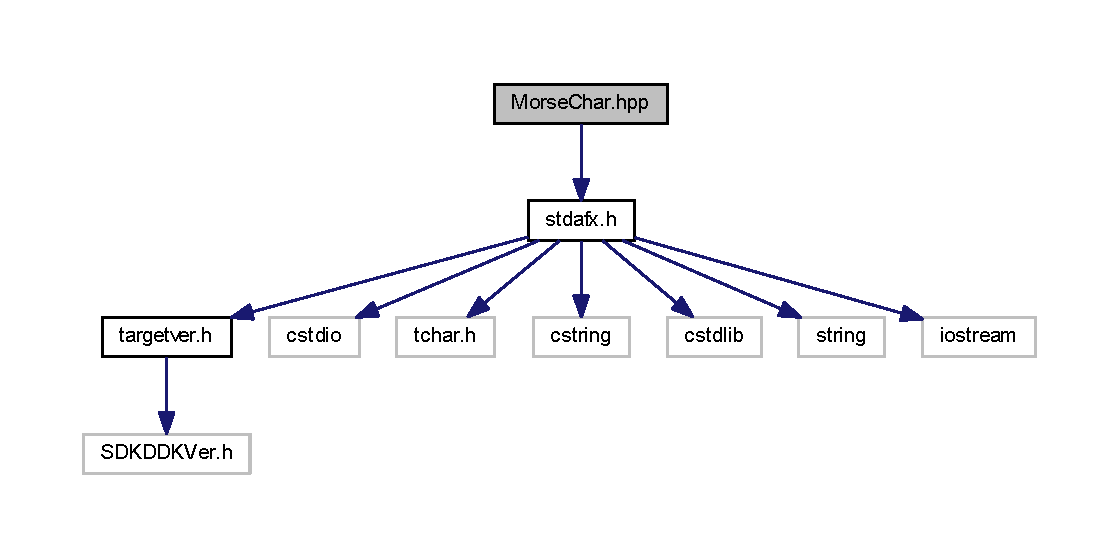
\includegraphics[width=350pt]{_morse_char_8hpp__incl}
\end{center}
\end{figure}
This graph shows which files directly or indirectly include this file\-:\nopagebreak
\begin{figure}[H]
\begin{center}
\leavevmode
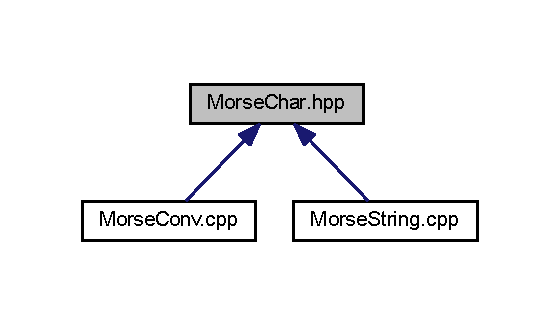
\includegraphics[width=269pt]{_morse_char_8hpp__dep__incl}
\end{center}
\end{figure}
\subsection*{Classes}
\begin{DoxyCompactItemize}
\item 
class \hyperlink{class_morse_char}{Morse\-Char}
\end{DoxyCompactItemize}

\hypertarget{_morse_conv_8cpp}{\section{Morse\-Conv.\-cpp File Reference}
\label{_morse_conv_8cpp}\index{Morse\-Conv.\-cpp@{Morse\-Conv.\-cpp}}
}
{\ttfamily \#include \char`\"{}stdafx.\-h\char`\"{}}\\*
{\ttfamily \#include \char`\"{}Morse\-Char.\-hpp\char`\"{}}\\*
{\ttfamily \#include \char`\"{}Morse\-String.\-hpp\char`\"{}}\\*
Include dependency graph for Morse\-Conv.\-cpp\-:\nopagebreak
\begin{figure}[H]
\begin{center}
\leavevmode
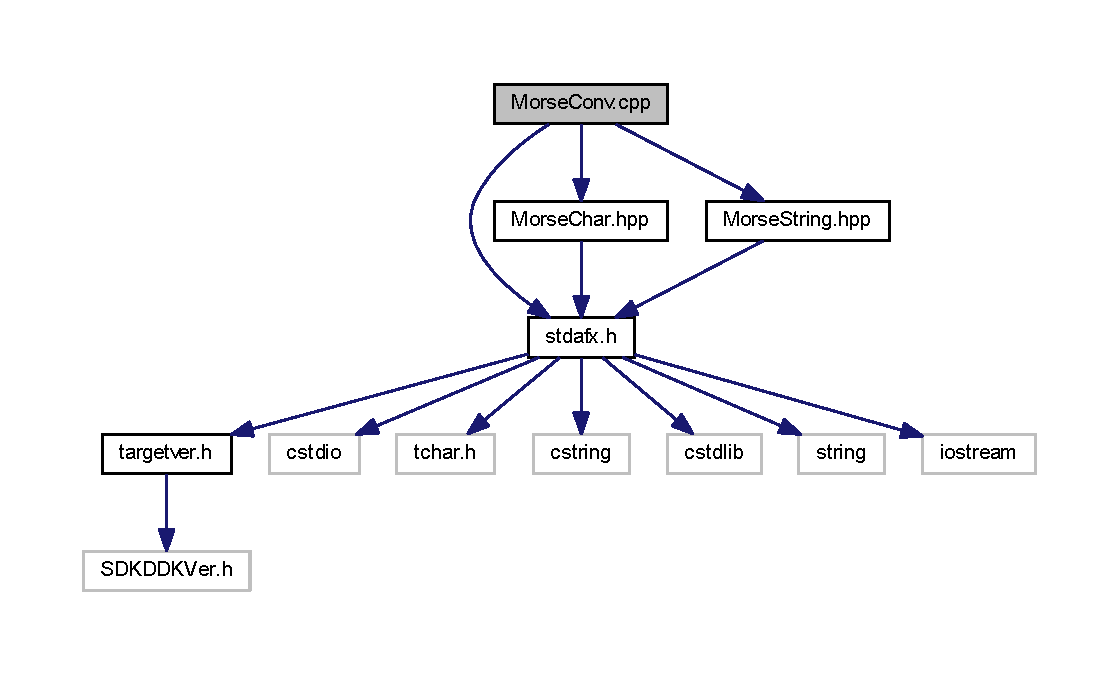
\includegraphics[width=350pt]{_morse_conv_8cpp__incl}
\end{center}
\end{figure}
\subsection*{Functions}
\begin{DoxyCompactItemize}
\item 
int \hyperlink{_morse_conv_8cpp_a0ddf1224851353fc92bfbff6f499fa97}{main} (int argc, char $\ast$argv\mbox{[}$\,$\mbox{]})
\end{DoxyCompactItemize}


\subsection{Function Documentation}
\hypertarget{_morse_conv_8cpp_a0ddf1224851353fc92bfbff6f499fa97}{\index{Morse\-Conv.\-cpp@{Morse\-Conv.\-cpp}!main@{main}}
\index{main@{main}!MorseConv.cpp@{Morse\-Conv.\-cpp}}
\subsubsection[{main}]{\setlength{\rightskip}{0pt plus 5cm}int main (
\begin{DoxyParamCaption}
\item[{int}]{argc, }
\item[{char $\ast$}]{argv\mbox{[}$\,$\mbox{]}}
\end{DoxyParamCaption}
)}}\label{_morse_conv_8cpp_a0ddf1224851353fc92bfbff6f499fa97}


Definition at line 23 of file Morse\-Conv.\-cpp.


\hypertarget{_morse_string_8cpp}{\section{Morse\-String.\-cpp File Reference}
\label{_morse_string_8cpp}\index{Morse\-String.\-cpp@{Morse\-String.\-cpp}}
}
{\ttfamily \#include \char`\"{}stdafx.\-h\char`\"{}}\\*
{\ttfamily \#include \char`\"{}Morse\-Char.\-hpp\char`\"{}}\\*
{\ttfamily \#include \char`\"{}Morse\-String.\-hpp\char`\"{}}\\*
Include dependency graph for Morse\-String.\-cpp\-:\nopagebreak
\begin{figure}[H]
\begin{center}
\leavevmode
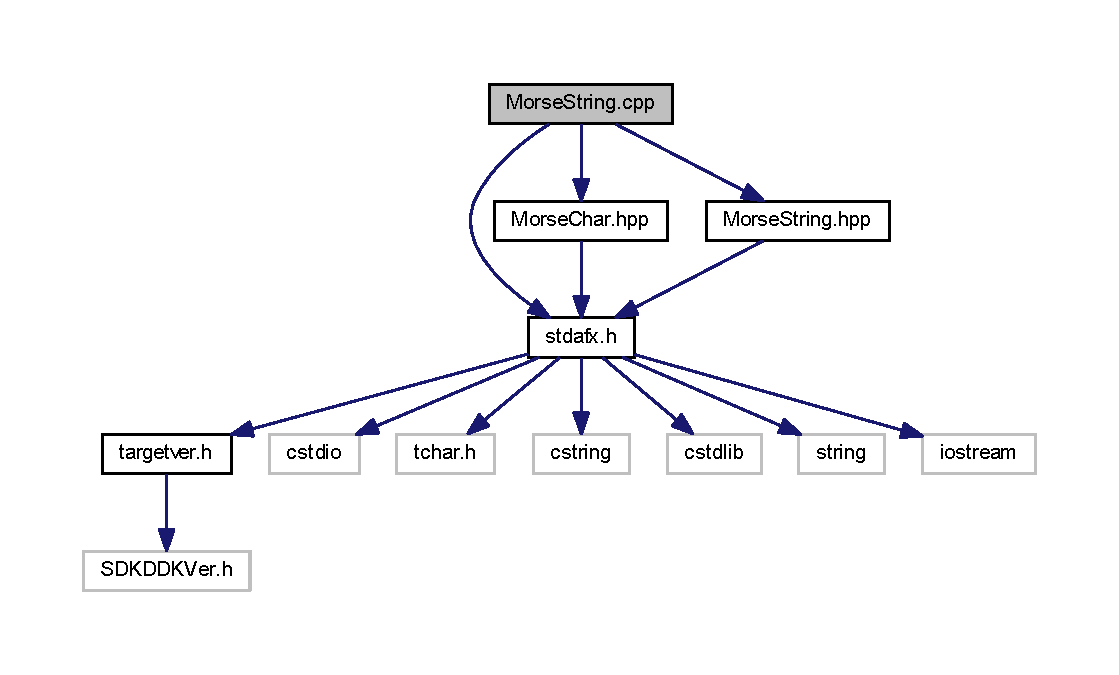
\includegraphics[width=350pt]{_morse_string_8cpp__incl}
\end{center}
\end{figure}
\subsection*{Macros}
\begin{DoxyCompactItemize}
\item 
\#define \hyperlink{_morse_string_8cpp_ac90cef74b3d8a53ffcc259acf1a9a1a1}{M\-O\-R\-S\-E\-\_\-\-A}~\char`\"{}.-\/\char`\"{}
\item 
\#define \hyperlink{_morse_string_8cpp_a6417446a0ea6bf49682cb7f87bac25b2}{M\-O\-R\-S\-E\-\_\-\-B}~\char`\"{}-\/...\char`\"{}
\item 
\#define \hyperlink{_morse_string_8cpp_a5b703140ac9b20639e597f693c5a1931}{M\-O\-R\-S\-E\-\_\-\-C}~\char`\"{}-\/.-\/.\char`\"{}
\item 
\#define \hyperlink{_morse_string_8cpp_a764d658e7abc257cdcda4911d48fa756}{M\-O\-R\-S\-E\-\_\-\-D}~\char`\"{}-\/..\char`\"{}
\item 
\#define \hyperlink{_morse_string_8cpp_a41d5921ee6ae595971cee43bff2853ae}{M\-O\-R\-S\-E\-\_\-\-E}~\char`\"{}.\char`\"{}
\item 
\#define \hyperlink{_morse_string_8cpp_aa5ab02d1b555d403d718cf9ba8f8c402}{M\-O\-R\-S\-E\-\_\-\-F}~\char`\"{}..-\/.\char`\"{}
\item 
\#define \hyperlink{_morse_string_8cpp_a20b208e9c719fdf8bd52496eb32a540e}{M\-O\-R\-S\-E\-\_\-\-G}~\char`\"{}-\/-\/.\char`\"{}
\item 
\#define \hyperlink{_morse_string_8cpp_ad877640af80edd6fa1e753f9a9a6e1dc}{M\-O\-R\-S\-E\-\_\-\-H}~\char`\"{}....\char`\"{}
\item 
\#define \hyperlink{_morse_string_8cpp_add0992c0b898a63f69ee0cc4b2eaf83f}{M\-O\-R\-S\-E\-\_\-\-I}~\char`\"{}..\char`\"{}
\item 
\#define \hyperlink{_morse_string_8cpp_ab8894d255f9747ad742a57ecb7b7e3ec}{M\-O\-R\-S\-E\-\_\-\-J}~\char`\"{}.-\/-\/-\/\char`\"{}
\item 
\#define \hyperlink{_morse_string_8cpp_a29c77d5610f319ddc54301c92c20511a}{M\-O\-R\-S\-E\-\_\-\-K}~\char`\"{}-\/.-\/\char`\"{}
\item 
\#define \hyperlink{_morse_string_8cpp_a9e1dc5bcaea248c4e9f70de78f6b0ca7}{M\-O\-R\-S\-E\-\_\-\-L}~\char`\"{}.-\/..\char`\"{}
\item 
\#define \hyperlink{_morse_string_8cpp_af6b475afc5ae4d3cdd4a6952cb4b26b8}{M\-O\-R\-S\-E\-\_\-\-M}~\char`\"{}-\/-\/\char`\"{}
\item 
\#define \hyperlink{_morse_string_8cpp_a78b7e075a081b21f8fd44c9d501f7eb5}{M\-O\-R\-S\-E\-\_\-\-N}~\char`\"{}-\/.\char`\"{}
\item 
\#define \hyperlink{_morse_string_8cpp_ae60b8b6911ee1303ded3bc72b586d7b5}{M\-O\-R\-S\-E\-\_\-\-O}~\char`\"{}-\/-\/-\/\char`\"{}
\item 
\#define \hyperlink{_morse_string_8cpp_a95fcc7194fcf7f9137800aa4c54c3d10}{M\-O\-R\-S\-E\-\_\-\-P}~\char`\"{}.-\/-\/.\char`\"{}
\item 
\#define \hyperlink{_morse_string_8cpp_abb88b34141b603deab0d4c5d522191fc}{M\-O\-R\-S\-E\-\_\-\-Q}~\char`\"{}-\/-\/.-\/\char`\"{}
\item 
\#define \hyperlink{_morse_string_8cpp_a0e8cb93a6eab2ff44bd70fd4bc4a9e0f}{M\-O\-R\-S\-E\-\_\-\-R}~\char`\"{}.-\/.\char`\"{}
\item 
\#define \hyperlink{_morse_string_8cpp_a32edd184ab6f81cefc8963ac974aa020}{M\-O\-R\-S\-E\-\_\-\-S}~\char`\"{}...\char`\"{}
\item 
\#define \hyperlink{_morse_string_8cpp_a6b09880d224ea926ef6a11cd50e45c4a}{M\-O\-R\-S\-E\-\_\-\-T}~\char`\"{}-\/\char`\"{}
\item 
\#define \hyperlink{_morse_string_8cpp_a29aa60862d0ff25612f41729784d3c52}{M\-O\-R\-S\-E\-\_\-\-U}~\char`\"{}..-\/\char`\"{}
\item 
\#define \hyperlink{_morse_string_8cpp_a14e7eeb0cc40a0a49cf8abf632525f56}{M\-O\-R\-S\-E\-\_\-\-V}~\char`\"{}...-\/\char`\"{}
\item 
\#define \hyperlink{_morse_string_8cpp_a13b8777aa5ed04958b1c598eb8737523}{M\-O\-R\-S\-E\-\_\-\-W}~\char`\"{}.-\/-\/\char`\"{}
\item 
\#define \hyperlink{_morse_string_8cpp_a096b7935af3df5522669a0db65e3e1e6}{M\-O\-R\-S\-E\-\_\-\-X}~\char`\"{}-\/..-\/\char`\"{}
\item 
\#define \hyperlink{_morse_string_8cpp_ac16ffe1a95f8f5143ab346c50865c977}{M\-O\-R\-S\-E\-\_\-\-Y}~\char`\"{}-\/.-\/-\/\char`\"{}
\item 
\#define \hyperlink{_morse_string_8cpp_a17a04da6a4c1399490d37928ee9dbec8}{M\-O\-R\-S\-E\-\_\-\-Z}~\char`\"{}-\/-\/..\char`\"{}
\item 
\#define \hyperlink{_morse_string_8cpp_a0884d818fd867b927db48b080ec8039e}{M\-O\-R\-S\-E\-\_\-1}~\char`\"{}.-\/-\/-\/-\/\char`\"{}
\item 
\#define \hyperlink{_morse_string_8cpp_af050c701815b8e9ed4520bc74fd2a56e}{M\-O\-R\-S\-E\-\_\-2}~\char`\"{}..-\/-\/-\/\char`\"{}
\item 
\#define \hyperlink{_morse_string_8cpp_acd51c5739777ff26baf0b7b76cb1c58a}{M\-O\-R\-S\-E\-\_\-3}~\char`\"{}...-\/-\/\char`\"{}
\item 
\#define \hyperlink{_morse_string_8cpp_ad012e9ea4e570878e5e7828afaf8fcd1}{M\-O\-R\-S\-E\-\_\-4}~\char`\"{}....-\/\char`\"{}
\item 
\#define \hyperlink{_morse_string_8cpp_a463792f3522dc011b9182d2324ff48d5}{M\-O\-R\-S\-E\-\_\-5}~\char`\"{}.....\char`\"{}
\item 
\#define \hyperlink{_morse_string_8cpp_adeebaca7d259f26eaa0faecbb586c77d}{M\-O\-R\-S\-E\-\_\-6}~\char`\"{}-\/....\char`\"{}
\item 
\#define \hyperlink{_morse_string_8cpp_a277f1840a7c4945516c03dfb573636bc}{M\-O\-R\-S\-E\-\_\-7}~\char`\"{}-\/-\/...\char`\"{}
\item 
\#define \hyperlink{_morse_string_8cpp_a66f2c7532f03b0c9de2105789abced9c}{M\-O\-R\-S\-E\-\_\-8}~\char`\"{}-\/-\/-\/..\char`\"{}
\item 
\#define \hyperlink{_morse_string_8cpp_a252ee8fd8541aa5ddab3b0fe29fb30e6}{M\-O\-R\-S\-E\-\_\-9}~\char`\"{}-\/-\/-\/-\/.\char`\"{}
\item 
\#define \hyperlink{_morse_string_8cpp_aa244c1442fffa5f80e3792406f7af69f}{M\-O\-R\-S\-E\-\_\-0}~\char`\"{}-\/-\/-\/-\/-\/\char`\"{}
\item 
\#define \hyperlink{_morse_string_8cpp_a19e2eb48c07c7148953daa3879d28b65}{M\-O\-R\-S\-E\-\_\-\-S\-P\-A\-C\-E}~\char`\"{} \char`\"{}
\item 
\#define \hyperlink{_morse_string_8cpp_a64273f3d8937b1830ddb60da07f78cee}{\-\_\-\-\_\-\-M\-O\-R\-S\-E\-\_\-\-D\-E\-F}(C)~M\-O\-R\-S\-E\-\_\- \#\# C
\item 
\#define \hyperlink{_morse_string_8cpp_afe942c2ccaf9ea890940ee6fd8f3d71e}{M\-O\-R\-S\-E\-\_\-\-P\-A\-R\-A\-M\-S}(C)~\hyperlink{_morse_string_8cpp_a64273f3d8937b1830ddb60da07f78cee}{\-\_\-\-\_\-\-M\-O\-R\-S\-E\-\_\-\-D\-E\-F}(C), sizeof(\hyperlink{_morse_string_8cpp_a64273f3d8937b1830ddb60da07f78cee}{\-\_\-\-\_\-\-M\-O\-R\-S\-E\-\_\-\-D\-E\-F}(C))
\end{DoxyCompactItemize}


\subsection{Macro Definition Documentation}
\hypertarget{_morse_string_8cpp_a64273f3d8937b1830ddb60da07f78cee}{\index{Morse\-String.\-cpp@{Morse\-String.\-cpp}!\-\_\-\-\_\-\-M\-O\-R\-S\-E\-\_\-\-D\-E\-F@{\-\_\-\-\_\-\-M\-O\-R\-S\-E\-\_\-\-D\-E\-F}}
\index{\-\_\-\-\_\-\-M\-O\-R\-S\-E\-\_\-\-D\-E\-F@{\-\_\-\-\_\-\-M\-O\-R\-S\-E\-\_\-\-D\-E\-F}!MorseString.cpp@{Morse\-String.\-cpp}}
\subsubsection[{\-\_\-\-\_\-\-M\-O\-R\-S\-E\-\_\-\-D\-E\-F}]{\setlength{\rightskip}{0pt plus 5cm}\#define \-\_\-\-\_\-\-M\-O\-R\-S\-E\-\_\-\-D\-E\-F(
\begin{DoxyParamCaption}
\item[{}]{C}
\end{DoxyParamCaption}
)~M\-O\-R\-S\-E\-\_\- \#\# C}}\label{_morse_string_8cpp_a64273f3d8937b1830ddb60da07f78cee}


Definition at line 61 of file Morse\-String.\-cpp.

\hypertarget{_morse_string_8cpp_aa244c1442fffa5f80e3792406f7af69f}{\index{Morse\-String.\-cpp@{Morse\-String.\-cpp}!M\-O\-R\-S\-E\-\_\-0@{M\-O\-R\-S\-E\-\_\-0}}
\index{M\-O\-R\-S\-E\-\_\-0@{M\-O\-R\-S\-E\-\_\-0}!MorseString.cpp@{Morse\-String.\-cpp}}
\subsubsection[{M\-O\-R\-S\-E\-\_\-0}]{\setlength{\rightskip}{0pt plus 5cm}\#define M\-O\-R\-S\-E\-\_\-0~\char`\"{}-\/-\/-\/-\/-\/\char`\"{}}}\label{_morse_string_8cpp_aa244c1442fffa5f80e3792406f7af69f}


Definition at line 58 of file Morse\-String.\-cpp.

\hypertarget{_morse_string_8cpp_a0884d818fd867b927db48b080ec8039e}{\index{Morse\-String.\-cpp@{Morse\-String.\-cpp}!M\-O\-R\-S\-E\-\_\-1@{M\-O\-R\-S\-E\-\_\-1}}
\index{M\-O\-R\-S\-E\-\_\-1@{M\-O\-R\-S\-E\-\_\-1}!MorseString.cpp@{Morse\-String.\-cpp}}
\subsubsection[{M\-O\-R\-S\-E\-\_\-1}]{\setlength{\rightskip}{0pt plus 5cm}\#define M\-O\-R\-S\-E\-\_\-1~\char`\"{}.-\/-\/-\/-\/\char`\"{}}}\label{_morse_string_8cpp_a0884d818fd867b927db48b080ec8039e}


Definition at line 49 of file Morse\-String.\-cpp.

\hypertarget{_morse_string_8cpp_af050c701815b8e9ed4520bc74fd2a56e}{\index{Morse\-String.\-cpp@{Morse\-String.\-cpp}!M\-O\-R\-S\-E\-\_\-2@{M\-O\-R\-S\-E\-\_\-2}}
\index{M\-O\-R\-S\-E\-\_\-2@{M\-O\-R\-S\-E\-\_\-2}!MorseString.cpp@{Morse\-String.\-cpp}}
\subsubsection[{M\-O\-R\-S\-E\-\_\-2}]{\setlength{\rightskip}{0pt plus 5cm}\#define M\-O\-R\-S\-E\-\_\-2~\char`\"{}..-\/-\/-\/\char`\"{}}}\label{_morse_string_8cpp_af050c701815b8e9ed4520bc74fd2a56e}


Definition at line 50 of file Morse\-String.\-cpp.

\hypertarget{_morse_string_8cpp_acd51c5739777ff26baf0b7b76cb1c58a}{\index{Morse\-String.\-cpp@{Morse\-String.\-cpp}!M\-O\-R\-S\-E\-\_\-3@{M\-O\-R\-S\-E\-\_\-3}}
\index{M\-O\-R\-S\-E\-\_\-3@{M\-O\-R\-S\-E\-\_\-3}!MorseString.cpp@{Morse\-String.\-cpp}}
\subsubsection[{M\-O\-R\-S\-E\-\_\-3}]{\setlength{\rightskip}{0pt plus 5cm}\#define M\-O\-R\-S\-E\-\_\-3~\char`\"{}...-\/-\/\char`\"{}}}\label{_morse_string_8cpp_acd51c5739777ff26baf0b7b76cb1c58a}


Definition at line 51 of file Morse\-String.\-cpp.

\hypertarget{_morse_string_8cpp_ad012e9ea4e570878e5e7828afaf8fcd1}{\index{Morse\-String.\-cpp@{Morse\-String.\-cpp}!M\-O\-R\-S\-E\-\_\-4@{M\-O\-R\-S\-E\-\_\-4}}
\index{M\-O\-R\-S\-E\-\_\-4@{M\-O\-R\-S\-E\-\_\-4}!MorseString.cpp@{Morse\-String.\-cpp}}
\subsubsection[{M\-O\-R\-S\-E\-\_\-4}]{\setlength{\rightskip}{0pt plus 5cm}\#define M\-O\-R\-S\-E\-\_\-4~\char`\"{}....-\/\char`\"{}}}\label{_morse_string_8cpp_ad012e9ea4e570878e5e7828afaf8fcd1}


Definition at line 52 of file Morse\-String.\-cpp.

\hypertarget{_morse_string_8cpp_a463792f3522dc011b9182d2324ff48d5}{\index{Morse\-String.\-cpp@{Morse\-String.\-cpp}!M\-O\-R\-S\-E\-\_\-5@{M\-O\-R\-S\-E\-\_\-5}}
\index{M\-O\-R\-S\-E\-\_\-5@{M\-O\-R\-S\-E\-\_\-5}!MorseString.cpp@{Morse\-String.\-cpp}}
\subsubsection[{M\-O\-R\-S\-E\-\_\-5}]{\setlength{\rightskip}{0pt plus 5cm}\#define M\-O\-R\-S\-E\-\_\-5~\char`\"{}.....\char`\"{}}}\label{_morse_string_8cpp_a463792f3522dc011b9182d2324ff48d5}


Definition at line 53 of file Morse\-String.\-cpp.

\hypertarget{_morse_string_8cpp_adeebaca7d259f26eaa0faecbb586c77d}{\index{Morse\-String.\-cpp@{Morse\-String.\-cpp}!M\-O\-R\-S\-E\-\_\-6@{M\-O\-R\-S\-E\-\_\-6}}
\index{M\-O\-R\-S\-E\-\_\-6@{M\-O\-R\-S\-E\-\_\-6}!MorseString.cpp@{Morse\-String.\-cpp}}
\subsubsection[{M\-O\-R\-S\-E\-\_\-6}]{\setlength{\rightskip}{0pt plus 5cm}\#define M\-O\-R\-S\-E\-\_\-6~\char`\"{}-\/....\char`\"{}}}\label{_morse_string_8cpp_adeebaca7d259f26eaa0faecbb586c77d}


Definition at line 54 of file Morse\-String.\-cpp.

\hypertarget{_morse_string_8cpp_a277f1840a7c4945516c03dfb573636bc}{\index{Morse\-String.\-cpp@{Morse\-String.\-cpp}!M\-O\-R\-S\-E\-\_\-7@{M\-O\-R\-S\-E\-\_\-7}}
\index{M\-O\-R\-S\-E\-\_\-7@{M\-O\-R\-S\-E\-\_\-7}!MorseString.cpp@{Morse\-String.\-cpp}}
\subsubsection[{M\-O\-R\-S\-E\-\_\-7}]{\setlength{\rightskip}{0pt plus 5cm}\#define M\-O\-R\-S\-E\-\_\-7~\char`\"{}-\/-\/...\char`\"{}}}\label{_morse_string_8cpp_a277f1840a7c4945516c03dfb573636bc}


Definition at line 55 of file Morse\-String.\-cpp.

\hypertarget{_morse_string_8cpp_a66f2c7532f03b0c9de2105789abced9c}{\index{Morse\-String.\-cpp@{Morse\-String.\-cpp}!M\-O\-R\-S\-E\-\_\-8@{M\-O\-R\-S\-E\-\_\-8}}
\index{M\-O\-R\-S\-E\-\_\-8@{M\-O\-R\-S\-E\-\_\-8}!MorseString.cpp@{Morse\-String.\-cpp}}
\subsubsection[{M\-O\-R\-S\-E\-\_\-8}]{\setlength{\rightskip}{0pt plus 5cm}\#define M\-O\-R\-S\-E\-\_\-8~\char`\"{}-\/-\/-\/..\char`\"{}}}\label{_morse_string_8cpp_a66f2c7532f03b0c9de2105789abced9c}


Definition at line 56 of file Morse\-String.\-cpp.

\hypertarget{_morse_string_8cpp_a252ee8fd8541aa5ddab3b0fe29fb30e6}{\index{Morse\-String.\-cpp@{Morse\-String.\-cpp}!M\-O\-R\-S\-E\-\_\-9@{M\-O\-R\-S\-E\-\_\-9}}
\index{M\-O\-R\-S\-E\-\_\-9@{M\-O\-R\-S\-E\-\_\-9}!MorseString.cpp@{Morse\-String.\-cpp}}
\subsubsection[{M\-O\-R\-S\-E\-\_\-9}]{\setlength{\rightskip}{0pt plus 5cm}\#define M\-O\-R\-S\-E\-\_\-9~\char`\"{}-\/-\/-\/-\/.\char`\"{}}}\label{_morse_string_8cpp_a252ee8fd8541aa5ddab3b0fe29fb30e6}


Definition at line 57 of file Morse\-String.\-cpp.

\hypertarget{_morse_string_8cpp_ac90cef74b3d8a53ffcc259acf1a9a1a1}{\index{Morse\-String.\-cpp@{Morse\-String.\-cpp}!M\-O\-R\-S\-E\-\_\-\-A@{M\-O\-R\-S\-E\-\_\-\-A}}
\index{M\-O\-R\-S\-E\-\_\-\-A@{M\-O\-R\-S\-E\-\_\-\-A}!MorseString.cpp@{Morse\-String.\-cpp}}
\subsubsection[{M\-O\-R\-S\-E\-\_\-\-A}]{\setlength{\rightskip}{0pt plus 5cm}\#define M\-O\-R\-S\-E\-\_\-\-A~\char`\"{}.-\/\char`\"{}}}\label{_morse_string_8cpp_ac90cef74b3d8a53ffcc259acf1a9a1a1}


Definition at line 23 of file Morse\-String.\-cpp.

\hypertarget{_morse_string_8cpp_a6417446a0ea6bf49682cb7f87bac25b2}{\index{Morse\-String.\-cpp@{Morse\-String.\-cpp}!M\-O\-R\-S\-E\-\_\-\-B@{M\-O\-R\-S\-E\-\_\-\-B}}
\index{M\-O\-R\-S\-E\-\_\-\-B@{M\-O\-R\-S\-E\-\_\-\-B}!MorseString.cpp@{Morse\-String.\-cpp}}
\subsubsection[{M\-O\-R\-S\-E\-\_\-\-B}]{\setlength{\rightskip}{0pt plus 5cm}\#define M\-O\-R\-S\-E\-\_\-\-B~\char`\"{}-\/...\char`\"{}}}\label{_morse_string_8cpp_a6417446a0ea6bf49682cb7f87bac25b2}


Definition at line 24 of file Morse\-String.\-cpp.

\hypertarget{_morse_string_8cpp_a5b703140ac9b20639e597f693c5a1931}{\index{Morse\-String.\-cpp@{Morse\-String.\-cpp}!M\-O\-R\-S\-E\-\_\-\-C@{M\-O\-R\-S\-E\-\_\-\-C}}
\index{M\-O\-R\-S\-E\-\_\-\-C@{M\-O\-R\-S\-E\-\_\-\-C}!MorseString.cpp@{Morse\-String.\-cpp}}
\subsubsection[{M\-O\-R\-S\-E\-\_\-\-C}]{\setlength{\rightskip}{0pt plus 5cm}\#define M\-O\-R\-S\-E\-\_\-\-C~\char`\"{}-\/.-\/.\char`\"{}}}\label{_morse_string_8cpp_a5b703140ac9b20639e597f693c5a1931}


Definition at line 25 of file Morse\-String.\-cpp.

\hypertarget{_morse_string_8cpp_a764d658e7abc257cdcda4911d48fa756}{\index{Morse\-String.\-cpp@{Morse\-String.\-cpp}!M\-O\-R\-S\-E\-\_\-\-D@{M\-O\-R\-S\-E\-\_\-\-D}}
\index{M\-O\-R\-S\-E\-\_\-\-D@{M\-O\-R\-S\-E\-\_\-\-D}!MorseString.cpp@{Morse\-String.\-cpp}}
\subsubsection[{M\-O\-R\-S\-E\-\_\-\-D}]{\setlength{\rightskip}{0pt plus 5cm}\#define M\-O\-R\-S\-E\-\_\-\-D~\char`\"{}-\/..\char`\"{}}}\label{_morse_string_8cpp_a764d658e7abc257cdcda4911d48fa756}


Definition at line 26 of file Morse\-String.\-cpp.

\hypertarget{_morse_string_8cpp_a41d5921ee6ae595971cee43bff2853ae}{\index{Morse\-String.\-cpp@{Morse\-String.\-cpp}!M\-O\-R\-S\-E\-\_\-\-E@{M\-O\-R\-S\-E\-\_\-\-E}}
\index{M\-O\-R\-S\-E\-\_\-\-E@{M\-O\-R\-S\-E\-\_\-\-E}!MorseString.cpp@{Morse\-String.\-cpp}}
\subsubsection[{M\-O\-R\-S\-E\-\_\-\-E}]{\setlength{\rightskip}{0pt plus 5cm}\#define M\-O\-R\-S\-E\-\_\-\-E~\char`\"{}.\char`\"{}}}\label{_morse_string_8cpp_a41d5921ee6ae595971cee43bff2853ae}


Definition at line 27 of file Morse\-String.\-cpp.

\hypertarget{_morse_string_8cpp_aa5ab02d1b555d403d718cf9ba8f8c402}{\index{Morse\-String.\-cpp@{Morse\-String.\-cpp}!M\-O\-R\-S\-E\-\_\-\-F@{M\-O\-R\-S\-E\-\_\-\-F}}
\index{M\-O\-R\-S\-E\-\_\-\-F@{M\-O\-R\-S\-E\-\_\-\-F}!MorseString.cpp@{Morse\-String.\-cpp}}
\subsubsection[{M\-O\-R\-S\-E\-\_\-\-F}]{\setlength{\rightskip}{0pt plus 5cm}\#define M\-O\-R\-S\-E\-\_\-\-F~\char`\"{}..-\/.\char`\"{}}}\label{_morse_string_8cpp_aa5ab02d1b555d403d718cf9ba8f8c402}


Definition at line 28 of file Morse\-String.\-cpp.

\hypertarget{_morse_string_8cpp_a20b208e9c719fdf8bd52496eb32a540e}{\index{Morse\-String.\-cpp@{Morse\-String.\-cpp}!M\-O\-R\-S\-E\-\_\-\-G@{M\-O\-R\-S\-E\-\_\-\-G}}
\index{M\-O\-R\-S\-E\-\_\-\-G@{M\-O\-R\-S\-E\-\_\-\-G}!MorseString.cpp@{Morse\-String.\-cpp}}
\subsubsection[{M\-O\-R\-S\-E\-\_\-\-G}]{\setlength{\rightskip}{0pt plus 5cm}\#define M\-O\-R\-S\-E\-\_\-\-G~\char`\"{}-\/-\/.\char`\"{}}}\label{_morse_string_8cpp_a20b208e9c719fdf8bd52496eb32a540e}


Definition at line 29 of file Morse\-String.\-cpp.

\hypertarget{_morse_string_8cpp_ad877640af80edd6fa1e753f9a9a6e1dc}{\index{Morse\-String.\-cpp@{Morse\-String.\-cpp}!M\-O\-R\-S\-E\-\_\-\-H@{M\-O\-R\-S\-E\-\_\-\-H}}
\index{M\-O\-R\-S\-E\-\_\-\-H@{M\-O\-R\-S\-E\-\_\-\-H}!MorseString.cpp@{Morse\-String.\-cpp}}
\subsubsection[{M\-O\-R\-S\-E\-\_\-\-H}]{\setlength{\rightskip}{0pt plus 5cm}\#define M\-O\-R\-S\-E\-\_\-\-H~\char`\"{}....\char`\"{}}}\label{_morse_string_8cpp_ad877640af80edd6fa1e753f9a9a6e1dc}


Definition at line 30 of file Morse\-String.\-cpp.

\hypertarget{_morse_string_8cpp_add0992c0b898a63f69ee0cc4b2eaf83f}{\index{Morse\-String.\-cpp@{Morse\-String.\-cpp}!M\-O\-R\-S\-E\-\_\-\-I@{M\-O\-R\-S\-E\-\_\-\-I}}
\index{M\-O\-R\-S\-E\-\_\-\-I@{M\-O\-R\-S\-E\-\_\-\-I}!MorseString.cpp@{Morse\-String.\-cpp}}
\subsubsection[{M\-O\-R\-S\-E\-\_\-\-I}]{\setlength{\rightskip}{0pt plus 5cm}\#define M\-O\-R\-S\-E\-\_\-\-I~\char`\"{}..\char`\"{}}}\label{_morse_string_8cpp_add0992c0b898a63f69ee0cc4b2eaf83f}


Definition at line 31 of file Morse\-String.\-cpp.

\hypertarget{_morse_string_8cpp_ab8894d255f9747ad742a57ecb7b7e3ec}{\index{Morse\-String.\-cpp@{Morse\-String.\-cpp}!M\-O\-R\-S\-E\-\_\-\-J@{M\-O\-R\-S\-E\-\_\-\-J}}
\index{M\-O\-R\-S\-E\-\_\-\-J@{M\-O\-R\-S\-E\-\_\-\-J}!MorseString.cpp@{Morse\-String.\-cpp}}
\subsubsection[{M\-O\-R\-S\-E\-\_\-\-J}]{\setlength{\rightskip}{0pt plus 5cm}\#define M\-O\-R\-S\-E\-\_\-\-J~\char`\"{}.-\/-\/-\/\char`\"{}}}\label{_morse_string_8cpp_ab8894d255f9747ad742a57ecb7b7e3ec}


Definition at line 32 of file Morse\-String.\-cpp.

\hypertarget{_morse_string_8cpp_a29c77d5610f319ddc54301c92c20511a}{\index{Morse\-String.\-cpp@{Morse\-String.\-cpp}!M\-O\-R\-S\-E\-\_\-\-K@{M\-O\-R\-S\-E\-\_\-\-K}}
\index{M\-O\-R\-S\-E\-\_\-\-K@{M\-O\-R\-S\-E\-\_\-\-K}!MorseString.cpp@{Morse\-String.\-cpp}}
\subsubsection[{M\-O\-R\-S\-E\-\_\-\-K}]{\setlength{\rightskip}{0pt plus 5cm}\#define M\-O\-R\-S\-E\-\_\-\-K~\char`\"{}-\/.-\/\char`\"{}}}\label{_morse_string_8cpp_a29c77d5610f319ddc54301c92c20511a}


Definition at line 33 of file Morse\-String.\-cpp.

\hypertarget{_morse_string_8cpp_a9e1dc5bcaea248c4e9f70de78f6b0ca7}{\index{Morse\-String.\-cpp@{Morse\-String.\-cpp}!M\-O\-R\-S\-E\-\_\-\-L@{M\-O\-R\-S\-E\-\_\-\-L}}
\index{M\-O\-R\-S\-E\-\_\-\-L@{M\-O\-R\-S\-E\-\_\-\-L}!MorseString.cpp@{Morse\-String.\-cpp}}
\subsubsection[{M\-O\-R\-S\-E\-\_\-\-L}]{\setlength{\rightskip}{0pt plus 5cm}\#define M\-O\-R\-S\-E\-\_\-\-L~\char`\"{}.-\/..\char`\"{}}}\label{_morse_string_8cpp_a9e1dc5bcaea248c4e9f70de78f6b0ca7}


Definition at line 34 of file Morse\-String.\-cpp.

\hypertarget{_morse_string_8cpp_af6b475afc5ae4d3cdd4a6952cb4b26b8}{\index{Morse\-String.\-cpp@{Morse\-String.\-cpp}!M\-O\-R\-S\-E\-\_\-\-M@{M\-O\-R\-S\-E\-\_\-\-M}}
\index{M\-O\-R\-S\-E\-\_\-\-M@{M\-O\-R\-S\-E\-\_\-\-M}!MorseString.cpp@{Morse\-String.\-cpp}}
\subsubsection[{M\-O\-R\-S\-E\-\_\-\-M}]{\setlength{\rightskip}{0pt plus 5cm}\#define M\-O\-R\-S\-E\-\_\-\-M~\char`\"{}-\/-\/\char`\"{}}}\label{_morse_string_8cpp_af6b475afc5ae4d3cdd4a6952cb4b26b8}


Definition at line 35 of file Morse\-String.\-cpp.

\hypertarget{_morse_string_8cpp_a78b7e075a081b21f8fd44c9d501f7eb5}{\index{Morse\-String.\-cpp@{Morse\-String.\-cpp}!M\-O\-R\-S\-E\-\_\-\-N@{M\-O\-R\-S\-E\-\_\-\-N}}
\index{M\-O\-R\-S\-E\-\_\-\-N@{M\-O\-R\-S\-E\-\_\-\-N}!MorseString.cpp@{Morse\-String.\-cpp}}
\subsubsection[{M\-O\-R\-S\-E\-\_\-\-N}]{\setlength{\rightskip}{0pt plus 5cm}\#define M\-O\-R\-S\-E\-\_\-\-N~\char`\"{}-\/.\char`\"{}}}\label{_morse_string_8cpp_a78b7e075a081b21f8fd44c9d501f7eb5}


Definition at line 36 of file Morse\-String.\-cpp.

\hypertarget{_morse_string_8cpp_ae60b8b6911ee1303ded3bc72b586d7b5}{\index{Morse\-String.\-cpp@{Morse\-String.\-cpp}!M\-O\-R\-S\-E\-\_\-\-O@{M\-O\-R\-S\-E\-\_\-\-O}}
\index{M\-O\-R\-S\-E\-\_\-\-O@{M\-O\-R\-S\-E\-\_\-\-O}!MorseString.cpp@{Morse\-String.\-cpp}}
\subsubsection[{M\-O\-R\-S\-E\-\_\-\-O}]{\setlength{\rightskip}{0pt plus 5cm}\#define M\-O\-R\-S\-E\-\_\-\-O~\char`\"{}-\/-\/-\/\char`\"{}}}\label{_morse_string_8cpp_ae60b8b6911ee1303ded3bc72b586d7b5}


Definition at line 37 of file Morse\-String.\-cpp.

\hypertarget{_morse_string_8cpp_a95fcc7194fcf7f9137800aa4c54c3d10}{\index{Morse\-String.\-cpp@{Morse\-String.\-cpp}!M\-O\-R\-S\-E\-\_\-\-P@{M\-O\-R\-S\-E\-\_\-\-P}}
\index{M\-O\-R\-S\-E\-\_\-\-P@{M\-O\-R\-S\-E\-\_\-\-P}!MorseString.cpp@{Morse\-String.\-cpp}}
\subsubsection[{M\-O\-R\-S\-E\-\_\-\-P}]{\setlength{\rightskip}{0pt plus 5cm}\#define M\-O\-R\-S\-E\-\_\-\-P~\char`\"{}.-\/-\/.\char`\"{}}}\label{_morse_string_8cpp_a95fcc7194fcf7f9137800aa4c54c3d10}


Definition at line 38 of file Morse\-String.\-cpp.

\hypertarget{_morse_string_8cpp_afe942c2ccaf9ea890940ee6fd8f3d71e}{\index{Morse\-String.\-cpp@{Morse\-String.\-cpp}!M\-O\-R\-S\-E\-\_\-\-P\-A\-R\-A\-M\-S@{M\-O\-R\-S\-E\-\_\-\-P\-A\-R\-A\-M\-S}}
\index{M\-O\-R\-S\-E\-\_\-\-P\-A\-R\-A\-M\-S@{M\-O\-R\-S\-E\-\_\-\-P\-A\-R\-A\-M\-S}!MorseString.cpp@{Morse\-String.\-cpp}}
\subsubsection[{M\-O\-R\-S\-E\-\_\-\-P\-A\-R\-A\-M\-S}]{\setlength{\rightskip}{0pt plus 5cm}\#define M\-O\-R\-S\-E\-\_\-\-P\-A\-R\-A\-M\-S(
\begin{DoxyParamCaption}
\item[{}]{C}
\end{DoxyParamCaption}
)~{\bf \-\_\-\-\_\-\-M\-O\-R\-S\-E\-\_\-\-D\-E\-F}(C), sizeof({\bf \-\_\-\-\_\-\-M\-O\-R\-S\-E\-\_\-\-D\-E\-F}(C))}}\label{_morse_string_8cpp_afe942c2ccaf9ea890940ee6fd8f3d71e}


Definition at line 62 of file Morse\-String.\-cpp.

\hypertarget{_morse_string_8cpp_abb88b34141b603deab0d4c5d522191fc}{\index{Morse\-String.\-cpp@{Morse\-String.\-cpp}!M\-O\-R\-S\-E\-\_\-\-Q@{M\-O\-R\-S\-E\-\_\-\-Q}}
\index{M\-O\-R\-S\-E\-\_\-\-Q@{M\-O\-R\-S\-E\-\_\-\-Q}!MorseString.cpp@{Morse\-String.\-cpp}}
\subsubsection[{M\-O\-R\-S\-E\-\_\-\-Q}]{\setlength{\rightskip}{0pt plus 5cm}\#define M\-O\-R\-S\-E\-\_\-\-Q~\char`\"{}-\/-\/.-\/\char`\"{}}}\label{_morse_string_8cpp_abb88b34141b603deab0d4c5d522191fc}


Definition at line 39 of file Morse\-String.\-cpp.

\hypertarget{_morse_string_8cpp_a0e8cb93a6eab2ff44bd70fd4bc4a9e0f}{\index{Morse\-String.\-cpp@{Morse\-String.\-cpp}!M\-O\-R\-S\-E\-\_\-\-R@{M\-O\-R\-S\-E\-\_\-\-R}}
\index{M\-O\-R\-S\-E\-\_\-\-R@{M\-O\-R\-S\-E\-\_\-\-R}!MorseString.cpp@{Morse\-String.\-cpp}}
\subsubsection[{M\-O\-R\-S\-E\-\_\-\-R}]{\setlength{\rightskip}{0pt plus 5cm}\#define M\-O\-R\-S\-E\-\_\-\-R~\char`\"{}.-\/.\char`\"{}}}\label{_morse_string_8cpp_a0e8cb93a6eab2ff44bd70fd4bc4a9e0f}


Definition at line 40 of file Morse\-String.\-cpp.

\hypertarget{_morse_string_8cpp_a32edd184ab6f81cefc8963ac974aa020}{\index{Morse\-String.\-cpp@{Morse\-String.\-cpp}!M\-O\-R\-S\-E\-\_\-\-S@{M\-O\-R\-S\-E\-\_\-\-S}}
\index{M\-O\-R\-S\-E\-\_\-\-S@{M\-O\-R\-S\-E\-\_\-\-S}!MorseString.cpp@{Morse\-String.\-cpp}}
\subsubsection[{M\-O\-R\-S\-E\-\_\-\-S}]{\setlength{\rightskip}{0pt plus 5cm}\#define M\-O\-R\-S\-E\-\_\-\-S~\char`\"{}...\char`\"{}}}\label{_morse_string_8cpp_a32edd184ab6f81cefc8963ac974aa020}


Definition at line 41 of file Morse\-String.\-cpp.

\hypertarget{_morse_string_8cpp_a19e2eb48c07c7148953daa3879d28b65}{\index{Morse\-String.\-cpp@{Morse\-String.\-cpp}!M\-O\-R\-S\-E\-\_\-\-S\-P\-A\-C\-E@{M\-O\-R\-S\-E\-\_\-\-S\-P\-A\-C\-E}}
\index{M\-O\-R\-S\-E\-\_\-\-S\-P\-A\-C\-E@{M\-O\-R\-S\-E\-\_\-\-S\-P\-A\-C\-E}!MorseString.cpp@{Morse\-String.\-cpp}}
\subsubsection[{M\-O\-R\-S\-E\-\_\-\-S\-P\-A\-C\-E}]{\setlength{\rightskip}{0pt plus 5cm}\#define M\-O\-R\-S\-E\-\_\-\-S\-P\-A\-C\-E~\char`\"{} \char`\"{}}}\label{_morse_string_8cpp_a19e2eb48c07c7148953daa3879d28b65}


Definition at line 59 of file Morse\-String.\-cpp.

\hypertarget{_morse_string_8cpp_a6b09880d224ea926ef6a11cd50e45c4a}{\index{Morse\-String.\-cpp@{Morse\-String.\-cpp}!M\-O\-R\-S\-E\-\_\-\-T@{M\-O\-R\-S\-E\-\_\-\-T}}
\index{M\-O\-R\-S\-E\-\_\-\-T@{M\-O\-R\-S\-E\-\_\-\-T}!MorseString.cpp@{Morse\-String.\-cpp}}
\subsubsection[{M\-O\-R\-S\-E\-\_\-\-T}]{\setlength{\rightskip}{0pt plus 5cm}\#define M\-O\-R\-S\-E\-\_\-\-T~\char`\"{}-\/\char`\"{}}}\label{_morse_string_8cpp_a6b09880d224ea926ef6a11cd50e45c4a}


Definition at line 42 of file Morse\-String.\-cpp.

\hypertarget{_morse_string_8cpp_a29aa60862d0ff25612f41729784d3c52}{\index{Morse\-String.\-cpp@{Morse\-String.\-cpp}!M\-O\-R\-S\-E\-\_\-\-U@{M\-O\-R\-S\-E\-\_\-\-U}}
\index{M\-O\-R\-S\-E\-\_\-\-U@{M\-O\-R\-S\-E\-\_\-\-U}!MorseString.cpp@{Morse\-String.\-cpp}}
\subsubsection[{M\-O\-R\-S\-E\-\_\-\-U}]{\setlength{\rightskip}{0pt plus 5cm}\#define M\-O\-R\-S\-E\-\_\-\-U~\char`\"{}..-\/\char`\"{}}}\label{_morse_string_8cpp_a29aa60862d0ff25612f41729784d3c52}


Definition at line 43 of file Morse\-String.\-cpp.

\hypertarget{_morse_string_8cpp_a14e7eeb0cc40a0a49cf8abf632525f56}{\index{Morse\-String.\-cpp@{Morse\-String.\-cpp}!M\-O\-R\-S\-E\-\_\-\-V@{M\-O\-R\-S\-E\-\_\-\-V}}
\index{M\-O\-R\-S\-E\-\_\-\-V@{M\-O\-R\-S\-E\-\_\-\-V}!MorseString.cpp@{Morse\-String.\-cpp}}
\subsubsection[{M\-O\-R\-S\-E\-\_\-\-V}]{\setlength{\rightskip}{0pt plus 5cm}\#define M\-O\-R\-S\-E\-\_\-\-V~\char`\"{}...-\/\char`\"{}}}\label{_morse_string_8cpp_a14e7eeb0cc40a0a49cf8abf632525f56}


Definition at line 44 of file Morse\-String.\-cpp.

\hypertarget{_morse_string_8cpp_a13b8777aa5ed04958b1c598eb8737523}{\index{Morse\-String.\-cpp@{Morse\-String.\-cpp}!M\-O\-R\-S\-E\-\_\-\-W@{M\-O\-R\-S\-E\-\_\-\-W}}
\index{M\-O\-R\-S\-E\-\_\-\-W@{M\-O\-R\-S\-E\-\_\-\-W}!MorseString.cpp@{Morse\-String.\-cpp}}
\subsubsection[{M\-O\-R\-S\-E\-\_\-\-W}]{\setlength{\rightskip}{0pt plus 5cm}\#define M\-O\-R\-S\-E\-\_\-\-W~\char`\"{}.-\/-\/\char`\"{}}}\label{_morse_string_8cpp_a13b8777aa5ed04958b1c598eb8737523}


Definition at line 45 of file Morse\-String.\-cpp.

\hypertarget{_morse_string_8cpp_a096b7935af3df5522669a0db65e3e1e6}{\index{Morse\-String.\-cpp@{Morse\-String.\-cpp}!M\-O\-R\-S\-E\-\_\-\-X@{M\-O\-R\-S\-E\-\_\-\-X}}
\index{M\-O\-R\-S\-E\-\_\-\-X@{M\-O\-R\-S\-E\-\_\-\-X}!MorseString.cpp@{Morse\-String.\-cpp}}
\subsubsection[{M\-O\-R\-S\-E\-\_\-\-X}]{\setlength{\rightskip}{0pt plus 5cm}\#define M\-O\-R\-S\-E\-\_\-\-X~\char`\"{}-\/..-\/\char`\"{}}}\label{_morse_string_8cpp_a096b7935af3df5522669a0db65e3e1e6}


Definition at line 46 of file Morse\-String.\-cpp.

\hypertarget{_morse_string_8cpp_ac16ffe1a95f8f5143ab346c50865c977}{\index{Morse\-String.\-cpp@{Morse\-String.\-cpp}!M\-O\-R\-S\-E\-\_\-\-Y@{M\-O\-R\-S\-E\-\_\-\-Y}}
\index{M\-O\-R\-S\-E\-\_\-\-Y@{M\-O\-R\-S\-E\-\_\-\-Y}!MorseString.cpp@{Morse\-String.\-cpp}}
\subsubsection[{M\-O\-R\-S\-E\-\_\-\-Y}]{\setlength{\rightskip}{0pt plus 5cm}\#define M\-O\-R\-S\-E\-\_\-\-Y~\char`\"{}-\/.-\/-\/\char`\"{}}}\label{_morse_string_8cpp_ac16ffe1a95f8f5143ab346c50865c977}


Definition at line 47 of file Morse\-String.\-cpp.

\hypertarget{_morse_string_8cpp_a17a04da6a4c1399490d37928ee9dbec8}{\index{Morse\-String.\-cpp@{Morse\-String.\-cpp}!M\-O\-R\-S\-E\-\_\-\-Z@{M\-O\-R\-S\-E\-\_\-\-Z}}
\index{M\-O\-R\-S\-E\-\_\-\-Z@{M\-O\-R\-S\-E\-\_\-\-Z}!MorseString.cpp@{Morse\-String.\-cpp}}
\subsubsection[{M\-O\-R\-S\-E\-\_\-\-Z}]{\setlength{\rightskip}{0pt plus 5cm}\#define M\-O\-R\-S\-E\-\_\-\-Z~\char`\"{}-\/-\/..\char`\"{}}}\label{_morse_string_8cpp_a17a04da6a4c1399490d37928ee9dbec8}


Definition at line 48 of file Morse\-String.\-cpp.


\hypertarget{_morse_string_8hpp}{\section{Morse\-String.\-hpp File Reference}
\label{_morse_string_8hpp}\index{Morse\-String.\-hpp@{Morse\-String.\-hpp}}
}
{\ttfamily \#include \char`\"{}stdafx.\-h\char`\"{}}\\*
Include dependency graph for Morse\-String.\-hpp\-:\nopagebreak
\begin{figure}[H]
\begin{center}
\leavevmode
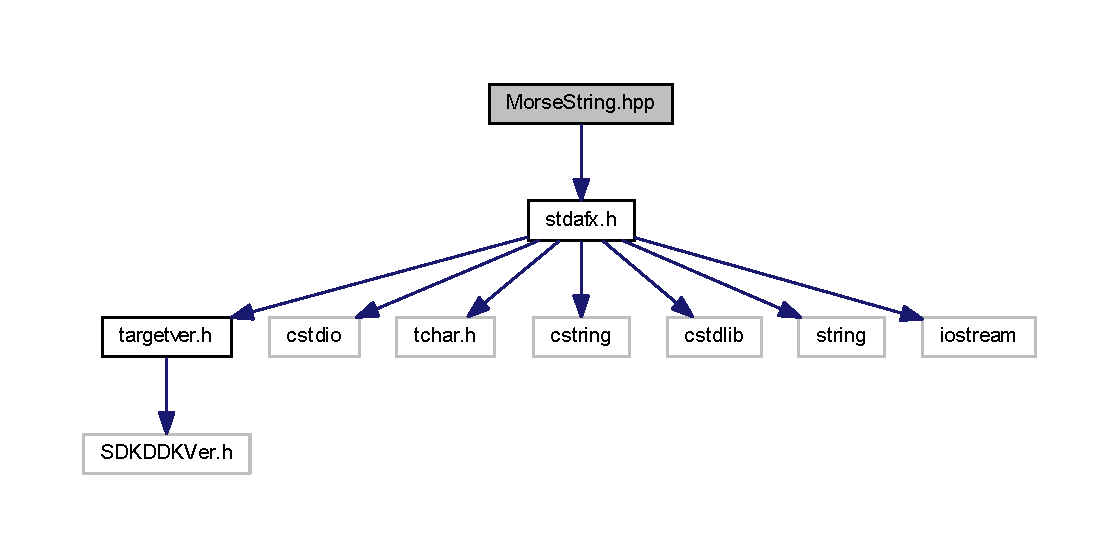
\includegraphics[width=350pt]{_morse_string_8hpp__incl}
\end{center}
\end{figure}
This graph shows which files directly or indirectly include this file\-:\nopagebreak
\begin{figure}[H]
\begin{center}
\leavevmode
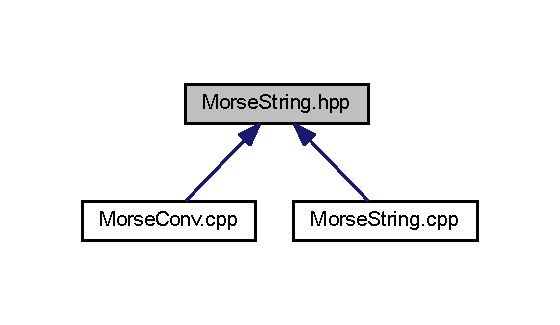
\includegraphics[width=269pt]{_morse_string_8hpp__dep__incl}
\end{center}
\end{figure}
\subsection*{Classes}
\begin{DoxyCompactItemize}
\item 
class \hyperlink{class_morse_string}{Morse\-String}
\item 
class \hyperlink{class_morse_string_1_1__iter}{Morse\-String\-::\-\_\-iter}
\end{DoxyCompactItemize}

\hypertarget{resource_8h}{\section{resource.\-h File Reference}
\label{resource_8h}\index{resource.\-h@{resource.\-h}}
}

\hypertarget{stdafx_8cpp}{\section{stdafx.\-cpp File Reference}
\label{stdafx_8cpp}\index{stdafx.\-cpp@{stdafx.\-cpp}}
}
{\ttfamily \#include \char`\"{}stdafx.\-h\char`\"{}}\\*
Include dependency graph for stdafx.\-cpp\-:\nopagebreak
\begin{figure}[H]
\begin{center}
\leavevmode
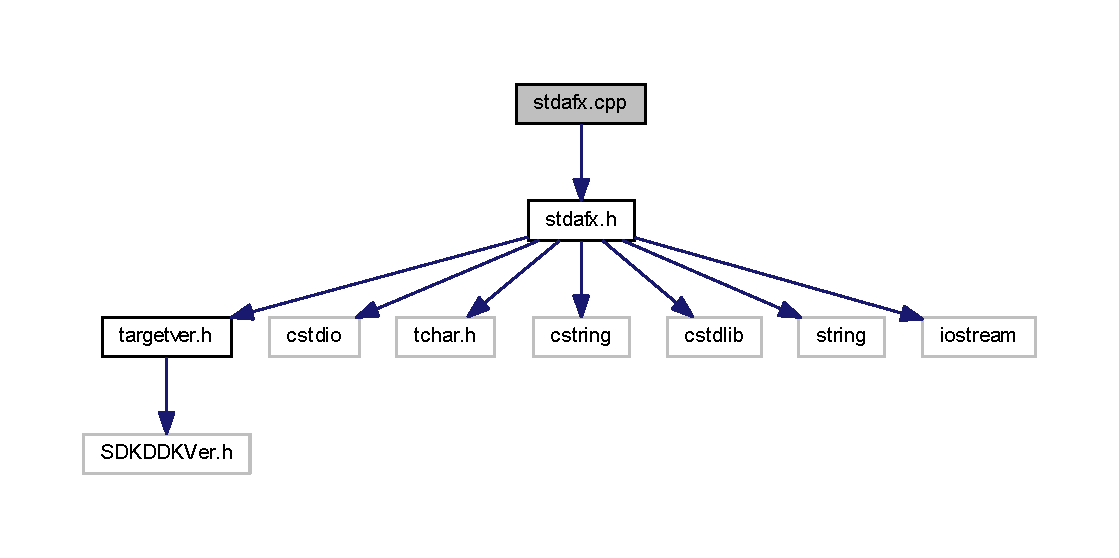
\includegraphics[width=350pt]{stdafx_8cpp__incl}
\end{center}
\end{figure}

\hypertarget{stdafx_8h}{\section{stdafx.\-h File Reference}
\label{stdafx_8h}\index{stdafx.\-h@{stdafx.\-h}}
}
{\ttfamily \#include \char`\"{}targetver.\-h\char`\"{}}\\*
{\ttfamily \#include $<$cstdio$>$}\\*
{\ttfamily \#include $<$tchar.\-h$>$}\\*
{\ttfamily \#include $<$cstring$>$}\\*
{\ttfamily \#include $<$cstdlib$>$}\\*
{\ttfamily \#include $<$string$>$}\\*
{\ttfamily \#include $<$iostream$>$}\\*
Include dependency graph for stdafx.\-h\-:\nopagebreak
\begin{figure}[H]
\begin{center}
\leavevmode
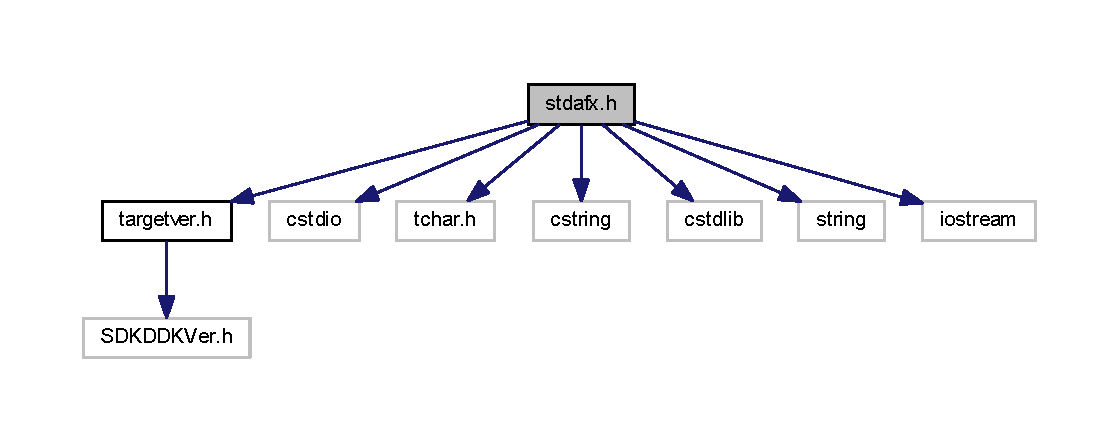
\includegraphics[width=350pt]{stdafx_8h__incl}
\end{center}
\end{figure}
This graph shows which files directly or indirectly include this file\-:\nopagebreak
\begin{figure}[H]
\begin{center}
\leavevmode
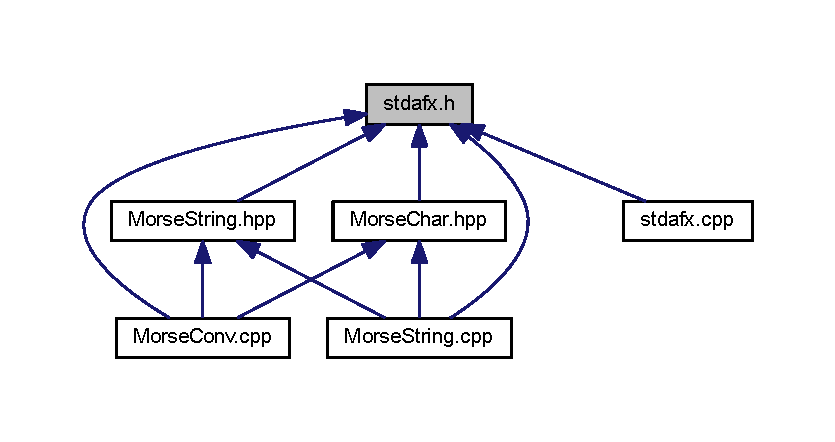
\includegraphics[width=350pt]{stdafx_8h__dep__incl}
\end{center}
\end{figure}

\hypertarget{targetver_8h}{\section{targetver.\-h File Reference}
\label{targetver_8h}\index{targetver.\-h@{targetver.\-h}}
}
{\ttfamily \#include $<$S\-D\-K\-D\-D\-K\-Ver.\-h$>$}\\*
Include dependency graph for targetver.\-h\-:\nopagebreak
\begin{figure}[H]
\begin{center}
\leavevmode
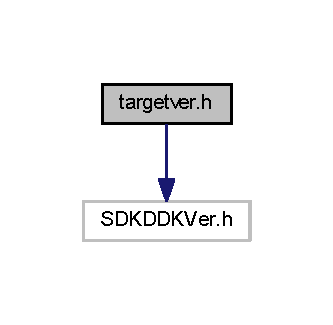
\includegraphics[width=160pt]{targetver_8h__incl}
\end{center}
\end{figure}
This graph shows which files directly or indirectly include this file\-:\nopagebreak
\begin{figure}[H]
\begin{center}
\leavevmode
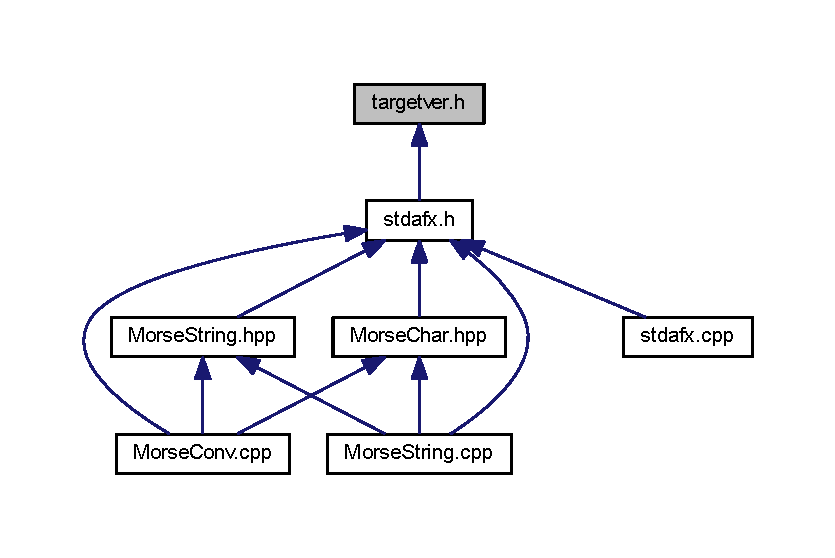
\includegraphics[width=350pt]{targetver_8h__dep__incl}
\end{center}
\end{figure}

%--- End generated contents ---

% Index
\newpage
\phantomsection
\addcontentsline{toc}{chapter}{Index}
\printindex

\end{document}
